\documentclass[a4paper,dutch]{article}

%% Language and font encodings
\usepackage[dutch]{babel}
\usepackage[utf8x]{inputenc}
\usepackage[T1]{fontenc}

%% Sets page size and margins
\usepackage[a4paper,top=3cm,bottom=2cm,left=3cm,right=3cm,marginparwidth=1.75cm]{geometry}
%\setlength{\parindent}{4em}
\setlength{\parskip}{1em}
%\renewcommand{\baselinestretch}{1.5}

%% Useful packages
\usepackage{amsmath}
%\usepackage{authblk}
\usepackage{graphicx}
\usepackage[colorinlistoftodos]{todonotes}
\usepackage[colorlinks=true, allcolors=blue]{hyperref}
\usepackage{pdfpages}
\usepackage[title]{appendix}
\usepackage{float}

\title{High efficiency LED stroboscoop}
\author{Bilican Mesut \and Boons Jarrit \and Gullentops Cédric}
%\affil{Departement Elektronica - ICT, Campus De Nayer}
\date{}

\begin{document}
\maketitle

\section{Inleiding}

Een stroboscoop is een optisch instrument waarmee de beweging van een draaiiend object schijnbaar kan worden stilgezet. Het effect ontstaat door de waarneming van het object slechts kortstondig toe te staan, steeds wanneer het object zich in dezelfde positie bevindt. Het oog mist de andere posities waardoor de illusie van stilstand ontstaat ~\cite{wiki:Stroboscoop}.%bron: Wikipedia

Onze opdracht was om een draagbaar autonoom toestel te bouwen dat lichtflitsen met instelbare frequentie en fase kan genereren via een power LED en dat in 2 modes kan werken:
\begin{itemize}
\item Frequentie mode waarbij de frequentie kan worden ingesteld tussen 0.1 HZ en 100 Hz in stappen van 0.1 Hz volgens het DDS principe\footnote{Direct digital synthesizer is het op digitale wijze opwekken van analoge signalen.}. %DDS uitleggen in footnote
\item Slave mode waarbij de frequentie gelijk of een veelvoud is van de frequentie aangebracht op de ingang, waarbij de faseverschuiving instelbaar is. Deze moest alleen in hardware geïmplementeerd worden.
\end{itemize}

De faseverschuiving kan ingesteld worden in de frequentie mode. De dutycycle en amplitude van de lichtimpulsen kan in beide modes ingesteld worden.

\section{Aanpak}
We hebben de stroboscoop verdeeld in kleine functionele blokken die je in figuur \ref{fig:simpel} kan zien.

We kozen voor de Arduino Micro als microcontroller vanwege de gebruiksvriendelijkheid, groot aantal poorten en beschikbaarheid van het product.

Voor de communicatie tussen gebruiker en toestel gebruiken we drukknoppen, een switch en een rotary encoder. Het LCD-scherm dient om de gekozen instellingen te tonen aan de gebruiker.

Als lichtbron kozen we een witte power LED die wordt aangedreven door een LED driver. De LED driver zorgt voor een constante stroom door onze power LED en heeft ook stroom- en temperatuurbeveiliging.

Om de autonomie van 3 uur te behalen kozen we voor een herlaadbare 3.6 V Li-ion batterij met een capaciteit van 2600 mAh en een circuit om de batterij op te laden.

Aangezien de batterij maar 3.6 V kan leveren en de output pinnen van de microcontroller maar 3.3 V en 5 V, moeten we d.m.v.\ DC-DC converters de spanningen 'boosten' naar de gewenste spanningen.

De onderverdeling van de uit te voeren taken vindt u in tabel \ref{tab:taakverdeling}.

\begin{table}
\centering
\begin{tabular}{l|l}
Student & Taken \\\hline
Mesut Bilican & probleemstelling oplossen, PCB-ontwerp, samenstellen PCB, testen \\
Jarrit Boons & probleemstelling oplossen,onderzoeken en uitwerken DDS en LED-aansturing, testen\\
Cédric Gullentops & probleemstelling oplossen, software design, programmeren van de software, testen\\
\end{tabular}
\caption{\label{tab:taakverdeling}De taakverdeling.}
\end{table}

\begin{figure}[htbp]
\centering
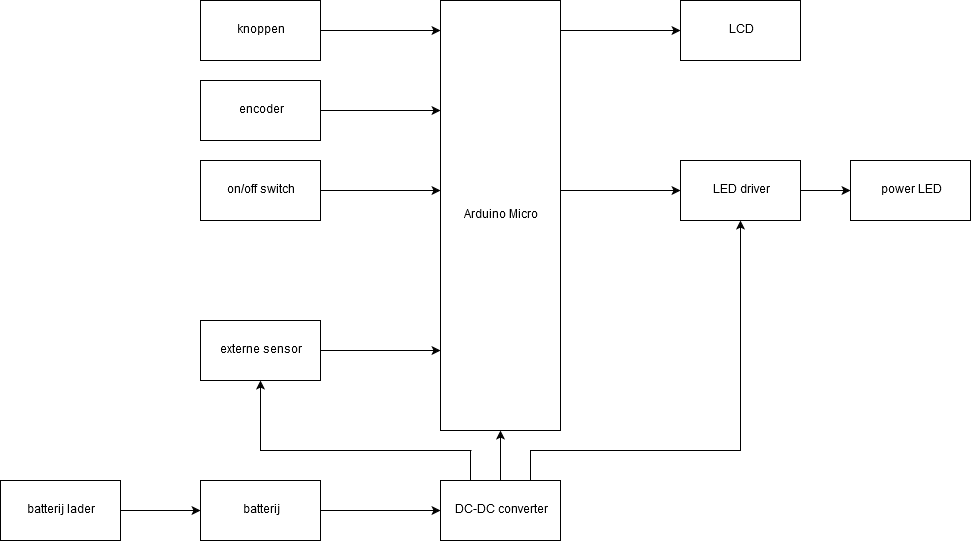
\includegraphics[width=1\textwidth]{simpel.png}
\caption{\label{fig:simpel}Blokschema stroboscoop.}
\end{figure}

\section{Planning}
\subsection{Tijdlijn}
\begin{figure}[H]
\centering
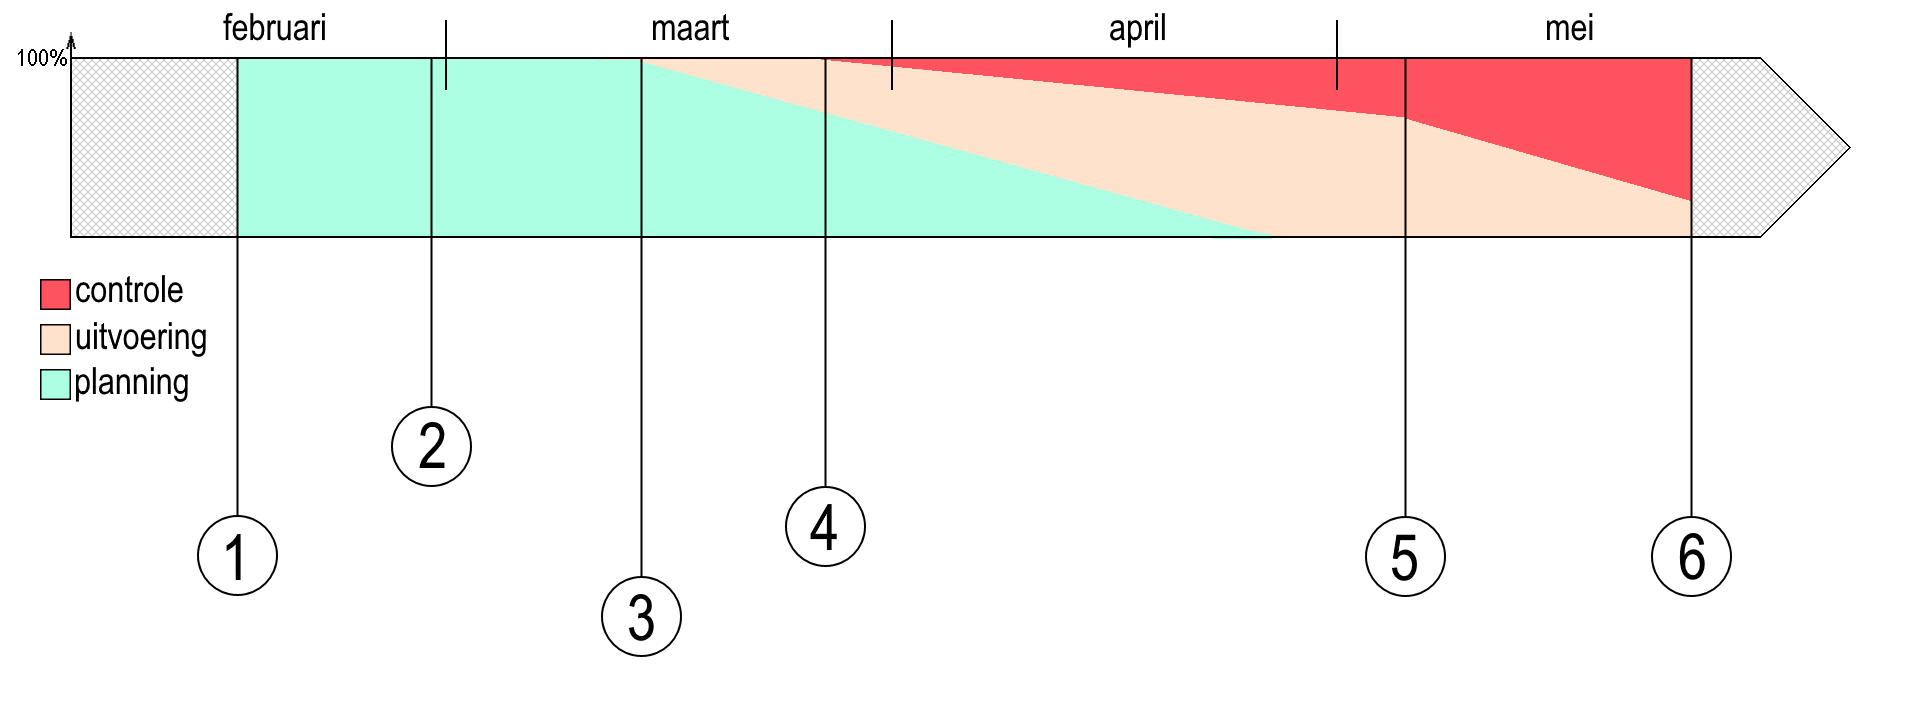
\includegraphics[width=\textwidth]{Timeline.png}
\caption{\label{fig:tijdlijn}Tijdlijn van projectvoortgang}
\end{figure}

\begin{enumerate}
\item (15/02): Keuze onderwerp + start project
\item (28/02): Taakverdeling + vooruitzichten gepland
\item (15/03): Lijst van componenten binnengeleverd, keuze van $\mu$-controller, beginnen met softwaregedeelte
\item (22/02): componenten aangekomen beginnen van softwaretests op arduino, ontbrekende of andere componenten bestellen
\item (06/05): Software klaar om te testen op breadboard, enkel nog kleine bugs, printplaat ontwerp klaar, laten afdrukken
\item (24/05): Deadline bachelorproef, presentatie
\end{enumerate}

Bovenstaande tijdlijn geeft het percentage van het soort werk dat in onze bachelor in die periode werd geïnvesteerd in functie van de tijd die we hadden om dit project uit te voeren, ongeveer 3.5 maanden. Ook staan de mijlpalen aangeduid en beschreven wat en wanneer we deze bereikt hebben. Deze waarden komen niet volledig overeen met diegene die we gepland hadden aan het begin van het semester, dit vaak door kleine setbacks of problemen met de levering. Wat opvalt is dat naarmate we verder in de tijd gaan het grootste aandeel eerst planning, dan uitvoering en ten slotte voornamelijk controle bedraagt. De kleuren veranderen echter niet abrupt maar lopen eerder in elkaar over. Zo valt het bijvoorbeeld op dat we tot eind april bezig waren met plannen, hoewel dit slechts een heel klein percentage is van de totale tijd. Het plannen was dan ook voornamelijk nog over dingen zoals het schriftelijke deel en de presentatie. Het grootste deel van de planning was gedaan eind maart, zodat ieders taak duidelijk was tijdens het paasverlof.

Normaal verwachten we dat op het einde van de periode uitvoering geen percentage meer zou innemen van de tijd. Dit is echter te wijten aan het feit dat er een foute inschatting was van het drukken van een printplaat waardoor er dingen last-minute moesten worden gedaan. Veel van onze tijd is dan ook verloren gegaan door het wachten op componenten waar we vaak merkten dat de eerder bestelde componenten niet deden wat er verwacht werd. 



Op het vlak van software hadden we dergelijke problemen niet omdat deze eenvoudig geschreven en getest kon worden met behulp van een breadboard en de reeds beschikbare componenten. Dit deel was dan ook relatief snel klaar, op enkele kleine maar lastige bugs na. Het was natuurlijk niet zeker of de code ook zou werken wanneer het geheel gesoldeerd was. 


\subsection{Struikelblokken}
Doorheen het project zijn we meerdere onvoorziene struikelblokken tegengekomen die onze planning door elkaar haalden of ons noodzaakte tot een andere aanpak:
\begin{itemize}
\item	Levertijden:\\
Een van de voornaamste struikelblokken waren de levertijden. We waren er ons vanaf aanvang van bewust dat we hiermee rekening moesten houden, maar dit bleek niet altijd te lukken. De tijd tussen een concept opstellen en dit werkelijk kunnen uitvoeren was vaak afhankelijk van de tijd dat de benodigde componenten geleverd konden worden. Deze tijd bedroeg gemiddeld 14 dagen waardoor telkens we een ander soort component moesten testen dit duurde meteen 2 weken langer dan verwacht. 

\item Design:\\
Het aanmaken van de componenten die niet in de libraries van Eagle zaten of niet geleverd werden door de fabrikant zorgde ervoor dat we zelf deze libraries moesten aanmaken.

Het plaatsen van de componenten en een goede lay-out maken nam ook veel tijd in beslag. Ook hadden we de afmetingen van sommige gaatjes voor de draden onderschat, waardoor we dun draad moesten gebruiken met als gevolg dat de draadjes snel afbreken of loskomen.
Een ander struikelblok was het aanmaken van de 'miniweerstanden'. Na veel opzoekwerk vonden we uiteindelijk dat we via het meander-commando lijnen konden meanderen zodat we de gewenste lengte konden behalen. 
Na een controle bleek dat er nog een paar dingen moest veranderd worden. De meeste dingen gingen vlot, maar met het veranderen van de lijndikte en het aanmaken van  via's naar de grondvlak voor de thermische eigenschappen van de LED driver hebben we niet snel kunnen oplossen. 

\item	Duurtijd:\\
We hebben enkele malen onderschat hoelang het geplande onderdeel daadwerkelijk duurde, op het vlak van software was dit niet extreem problematisch omdat dit vaak buiten de schooluren doenbaar was. Veel onderdelen die met hardware te maken hadden konden echter vaak enkel in de labo’s gedaan worden met als gevolg we achter geraakten op onze planning.

\item	Debugging:\\
Een groot onderdeel van code schrijven is het debuggen en testen van de geschreven software. Vooral wanneer meerdere routines samen worden gezet kunnen er onvoorspelbare errors optreden en het debuggen van deze loopt niet altijd van een leien dakje. Omdat dit echter buiten schooluren mogelijk was heeft het weinig invloed gehad op onze planning, maar wel een opmerkelijk aantal werkuren toegevoegd aan het project.

\item	Werking van componenten:\\
De werking van componenten staat vaak duidelijk beschreven in zijn datasheet. Sommige componenten hebben echter een minder overzichtelijke datasheet waardoor we de exacte werking slechts te weten kunnen komen door deze te testen. Wanneer ze dan niet naar verwachting functioneren dienden we een ander soort component te bestellen. Deze cyclus is erg tijdrovend en zorgde vaak voor onvoorziene vertragingen.

\item	Beschikbaarheid van componenten:\\
Het bestellen van componenten werd telkens via dezelfde leverancier, Farnell, gedaan.
Voor veel van onze projectonderdelen hadden we bij aanvang een concept in gedachten dat berustte op bepaalde componenten. Wanneer we opmerkte dat deze niet (meer) beschikbaar waren bij deze leverancier werden we genoodzaakt en nieuw concept op te stellen. Dit is meerdere malen voorgevallen waardoor we vaak concepten moesten herontwerpen of zelfs schrappen.

\end{itemize}



\section{Ontwerp}
\subsection{PCB}
Om de PCB te ontwerpen hebben we gebruik gemaakt van het Eagle softwarepakket. De gemaakte schema's en bijhorende PCB-lay-out zijn te vinden in  bijlage \ref{appendix:schema}, \ref{appendix:top} en \ref{appendix:bot}. 

\subsubsection{Berekeningen}
Om de juiste uitgangsspanning te verkrijgen uit de DC-DC converters hebben we de weerstanden als volgt berekent:

\[V_{out} = V_{TH} (\frac{R_2}{R_1} + 1)\]

met ${V_{TH}} = 1.25 \, V$.\\

Voor de 7 V converter kozen we voor $R_1 = 1 \, k\Omega$, hieruit volgt  $R_2 = 4.7 \, k\Omega$. $R_1$ en $R_2$ komen overeen met $R_1$ en $R_2$ in het schema (bijlage \ref{appendix:schema}). Voor de 24 V converter kozen we voor $R_1 = 1 \, k\Omega$ en  $R_2 = 18 \, k\Omega$ die overeenkomen met $R_3$ en $R_4$ respectievelijk. 

De weerstand bij de 5 V clipper hebben zo gekozen dat de stroom doorheen de zenerdiode van 5 V en de Arduino Micro $I_{max}$ niet overschrijdt. Met een ingangsspanning van 24 V komen we neer op een weerstand van $1 \,k\Omega$ voor een stroom van $20 \, mA$.

\begin{figure}[H]
\centering
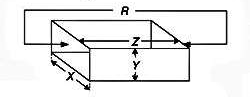
\includegraphics[width=0.5\textwidth]{resistance.png}
\caption{\label{fig:resistance}Dimensies koperfolie.}
\end{figure}

Zowel de DC-DC converter als de LED driver werken met heel kleine 'sense' weerstanden die we niet kunnen aankopen, maar als een koperfolie op de PCB moeten implementeren a.d.h.v.\ de soortelijke weerstand $\rho$. 
De soortelijke weerstand van koper bij 25 ºC is 724 x $10^{-6} \, Ωcm$. De dikte $Y$ van een standaard PCB koperfolie is 36 $\mu m$ ~\cite{ontwerp} (fig \ref{fig:resistance}).

De formule voor de weerstand is het volgende:

\[R_f=\frac{\rho Z}{X Y}\]

met $\rho = 724 x 10^{-6} \, Ωcm$, $Z = \text{lengte van folie}$, $X = \text{breedte van folie}$ en $Y = \text{dikte van folie}$.

Vereenvoudigt wordt dit
\[R_f=0.48 \frac{Z}{X} \, [m\Omega]\]

Voor de weerstand van $150\,m\Omega$ en de gebruikte foliebreedte van $20\,mils$ of $0.508\,mm$ komen we uit op een folielengte van $158.75\,mm$. Voor de weerstand van $286\,m\Omega$ krijgen we een folielengte van $302.68\,mm$ die we in kunnen Eagle implementeren.
% PCB design Pauwels linken bron

\subsection{Software}

We hebben als microprocessor gekozen voor de Arduino Micro. 
Het programmeren van de Arduino Micro wordt gedaan in C/C++ waarbij de focus ligt op C. Niet alles van C++ wordt namelijk door de compiler geaccepteerd. Arduino producten zijn open source, zowel qua software, als qua hardware. Het vinden van handige libraries is dus niet zo moeilijk. Wij hebben zelf ook gebruik gemaakt van enkele libraries zoals: LiquidCrystal voor de LCD, TimerOne voor de interrupt en RotaryEncoder voor de rotary encoder. Deze twee laatste maken geen deel uit van de standaardlibraries, u kan de links naar deze libraries vinden in de referenties ~\cite{Github:TimerOne} en ~\cite{mathertel:RotaryEncoder}. 

De Arduino bevat 32KB aan flash geheugen, waarvan 4KB gereserveerd wordt voor de bootloader. De overige 28KB zijn dus ter beschikking voor het programma. De arduino beschikt ook over 1KB EEPROM geheugen en 2,5KB SRAM. Het EEPROM wordt gebruikt voor variabelen een lange periode op te slagen en het SRAM wordt gebruikt om variabelen op te slaan en manipuleren tijdens runtime. In fig \ref{fig:memory map} ziet u een voorstelling van hoe dit er uitziet. 

\begin{figure}[H]
\centering
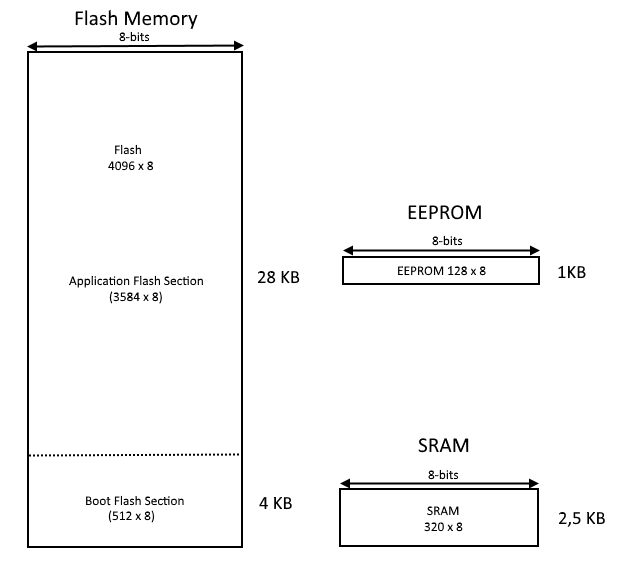
\includegraphics[width=0.5\textwidth]{Memory_Map.png}
\caption{\label{fig:memory map}Memory Map.}
\end{figure}

We zullen een korte beschrijving geven van de software door middel van pseudo-code en bijhordende figuren in de bijlage. We kunnen de software opdelen in 3 delen. Het eerste deel is de setup, deze functie wordt slechts eenmaal opgeroepen en bevat de meeste initialisaties van de variabelen zoals deze van de TimerOne interrupt en de LCD. Zie fig \ref{fig:setup}.

Het tweede deel is de loop-functie. Zie fig \ref{fig:loop}. Deze functie zal worden uitgevoerd na de setup-functie. De loop-functie, zoals de naam zegt, zal telkens opnieuw worden uitgevoerd. Eerst zullen button en switch presses gedetecteerd worden, hierna zal er worden gekeken in welke mode men zich bevindt. De frequentie mode is de standaard mode waarin eerst gecontroleerd wordt of er in de huidige iteratie aan de rotary encoder is gedraaid. Bij een draaiing zal 1 van de 5 variabelen aangepast kunnen worden. Ten slotte zal er worden gecontroleerd of een variabele is aangepast en in deze gevallen zal de lcd geupdate worden.Voor deze functie zie fig \ref{fig:lcd}. De alternatieve mode is de slave mode, helaas hebben we deze niet kunnen realiseren omdat we met een kleinere groep waren.

Het laatste deel is de interrupt functie, deze zal elke 100µs worden uitgevoerd. Zie fig \ref{fig:interrupt}. In de interrupt word een counter opgeteld tot de gewenste periode bereikt wordt waarna de LED van staat zal veranderen via de blinkLED-functie. Zie fig \ref{fig:blinkled}. Als in de loop-functie de fase verandert werd zal deze worden juist gezet via een andere teller in de interrupt en dan zal de huidige staat van de LED bewaard worden. Als de fase verandert in de loop-functie terwijl de counter al aan het tellen was zal de fasedraaiing al worden herrekend en dan wordt de counter gereset.

Ten slotte hebben we een variabel map gemaakt waarin een samenvatting staat van alle variabelen, hun type en een korte descriptie over hun functie. Ook deze kunt u zien op fig \ref{fig:varmap}.

\section{Testen en resultaten}

De software hebben we getest door de uitgang van de Arduino Micro te meten met een oscilloscoop. We hebben de verschillende mogelijkheden getest zoals frequentie, dutycycle en helderheid die te zien zijn in bijlage \ref{appendix:Testresultaten}. Faseverschuiving hebben we niet via de oscilloscoop kunnen verifiëren omdat de oscilloscoop telkens bij het verschuiven zich aanpast. We hebben de fase wel visueel kunnen testen via het onboard ledje van de Arduino. We kunnen zo echter wel niet zien dat de timing volledig correct is. 

De PCB hebben we getest door de batterij te vervangen door de labovoeding. 
De testen werden uitgevoerd op de ingang en uitgang van de converters, LED driver en de pinnen van componenten waarop we de spanning van wisten.

De eerste test gaf meteen al een fout aan. De uitgangsspanningen waren gelijk aan de aangelegde spanning. Dit kwam doordat het gaatje waarin de negatieve ingang van de batterij of voeding  kwam niet verbonden was met de grondvlak. Dit hebben we opgelost door een stukje van de grondvlak bloot te stellen en deze te verbinden met het gaatje.

De test hierna gaf aan dat het voorgaande probleem opgelost is.
De gemeten spanning aan de pinnen waren dit keer verschillend, maar we verkregen foute spanningen aan de uitgang. Na grondig bekijken van de PCB lay-out blijkt dat de connecties vanuit de pinnen 6 en 7 van de DC-DC converters omgewisseld waren. Dit komt doordat bij ons schema, dat in eerste instantie lijkt te kloppen, de omzetting naar PCB geen wordt rekening gehouden met de 'dummy' weerstand van 150 m$\Omega$. Het gevolg hiervan is dat pin 6 en 7 technisch gezien direct met elkaar verbonden zijn. Na het analyseren van de PCB hebben we vastgesteld dat het wisselen van pin 6 en 7 de gewenste oplossing biedt. Praktisch hebben we het opgelost door pin 6 en 7 om te leiden d.m.v. \ draadjes en koper weg te schrappen. 

Na de omleiding hebben we onze laatste test uitgevoerd. Ditmaal gaf de voeding kortsluiting  aan. We weten dat het iets met de omleiding te maken heeft, maar waar het probleem zich juist bevindt hebben we niet kunnen vinden.



\section{Besluit}
Uit de testen zien we dat onze software werkt. De verschillende mogelijkheden zoals het aanpassen van de frequentie, dutycycle, helderheid en fase is mogelijk met de rotary encoder in stappen van 0.1, 1 en 10.

De hardware aan de andere kant heeft een paar fouten. Allereerst hebben we de toggle-switch om het circuit aan en uit te zetten verkeerd geplaatst, maar met een paar draadjes kan dit eenvoudig opgelost worden. Ten tweede hadden we een probleem met de massa, die uiteindelijk niet met de grond verbonden was. Dit hebben we ook makkelijk kunnen oplossen door middel van een draadje te verbinden met een open vlakje aan de bodem. Het derde probleem dat we ondervonden hebben, was dat pin 6 en 7 van de DC-DC boost converter omgewisseld waren. Na het omwisselen van de pinnen zijn we helaas op een ander probleem gestuit. Namelijk dat er ergens rond de omgewisselde pinnen kortsluiting ontstaat. Helaas hebben we de oorzaak van de kortsluiting niet kunnen vinden.


\bibliographystyle{alpha}
\bibliography{sample}

\pagebreak

\begin{appendices}
\section{Testresultaten}
\label{appendix:Testresultaten}
\begin{figure}[H]
\centering
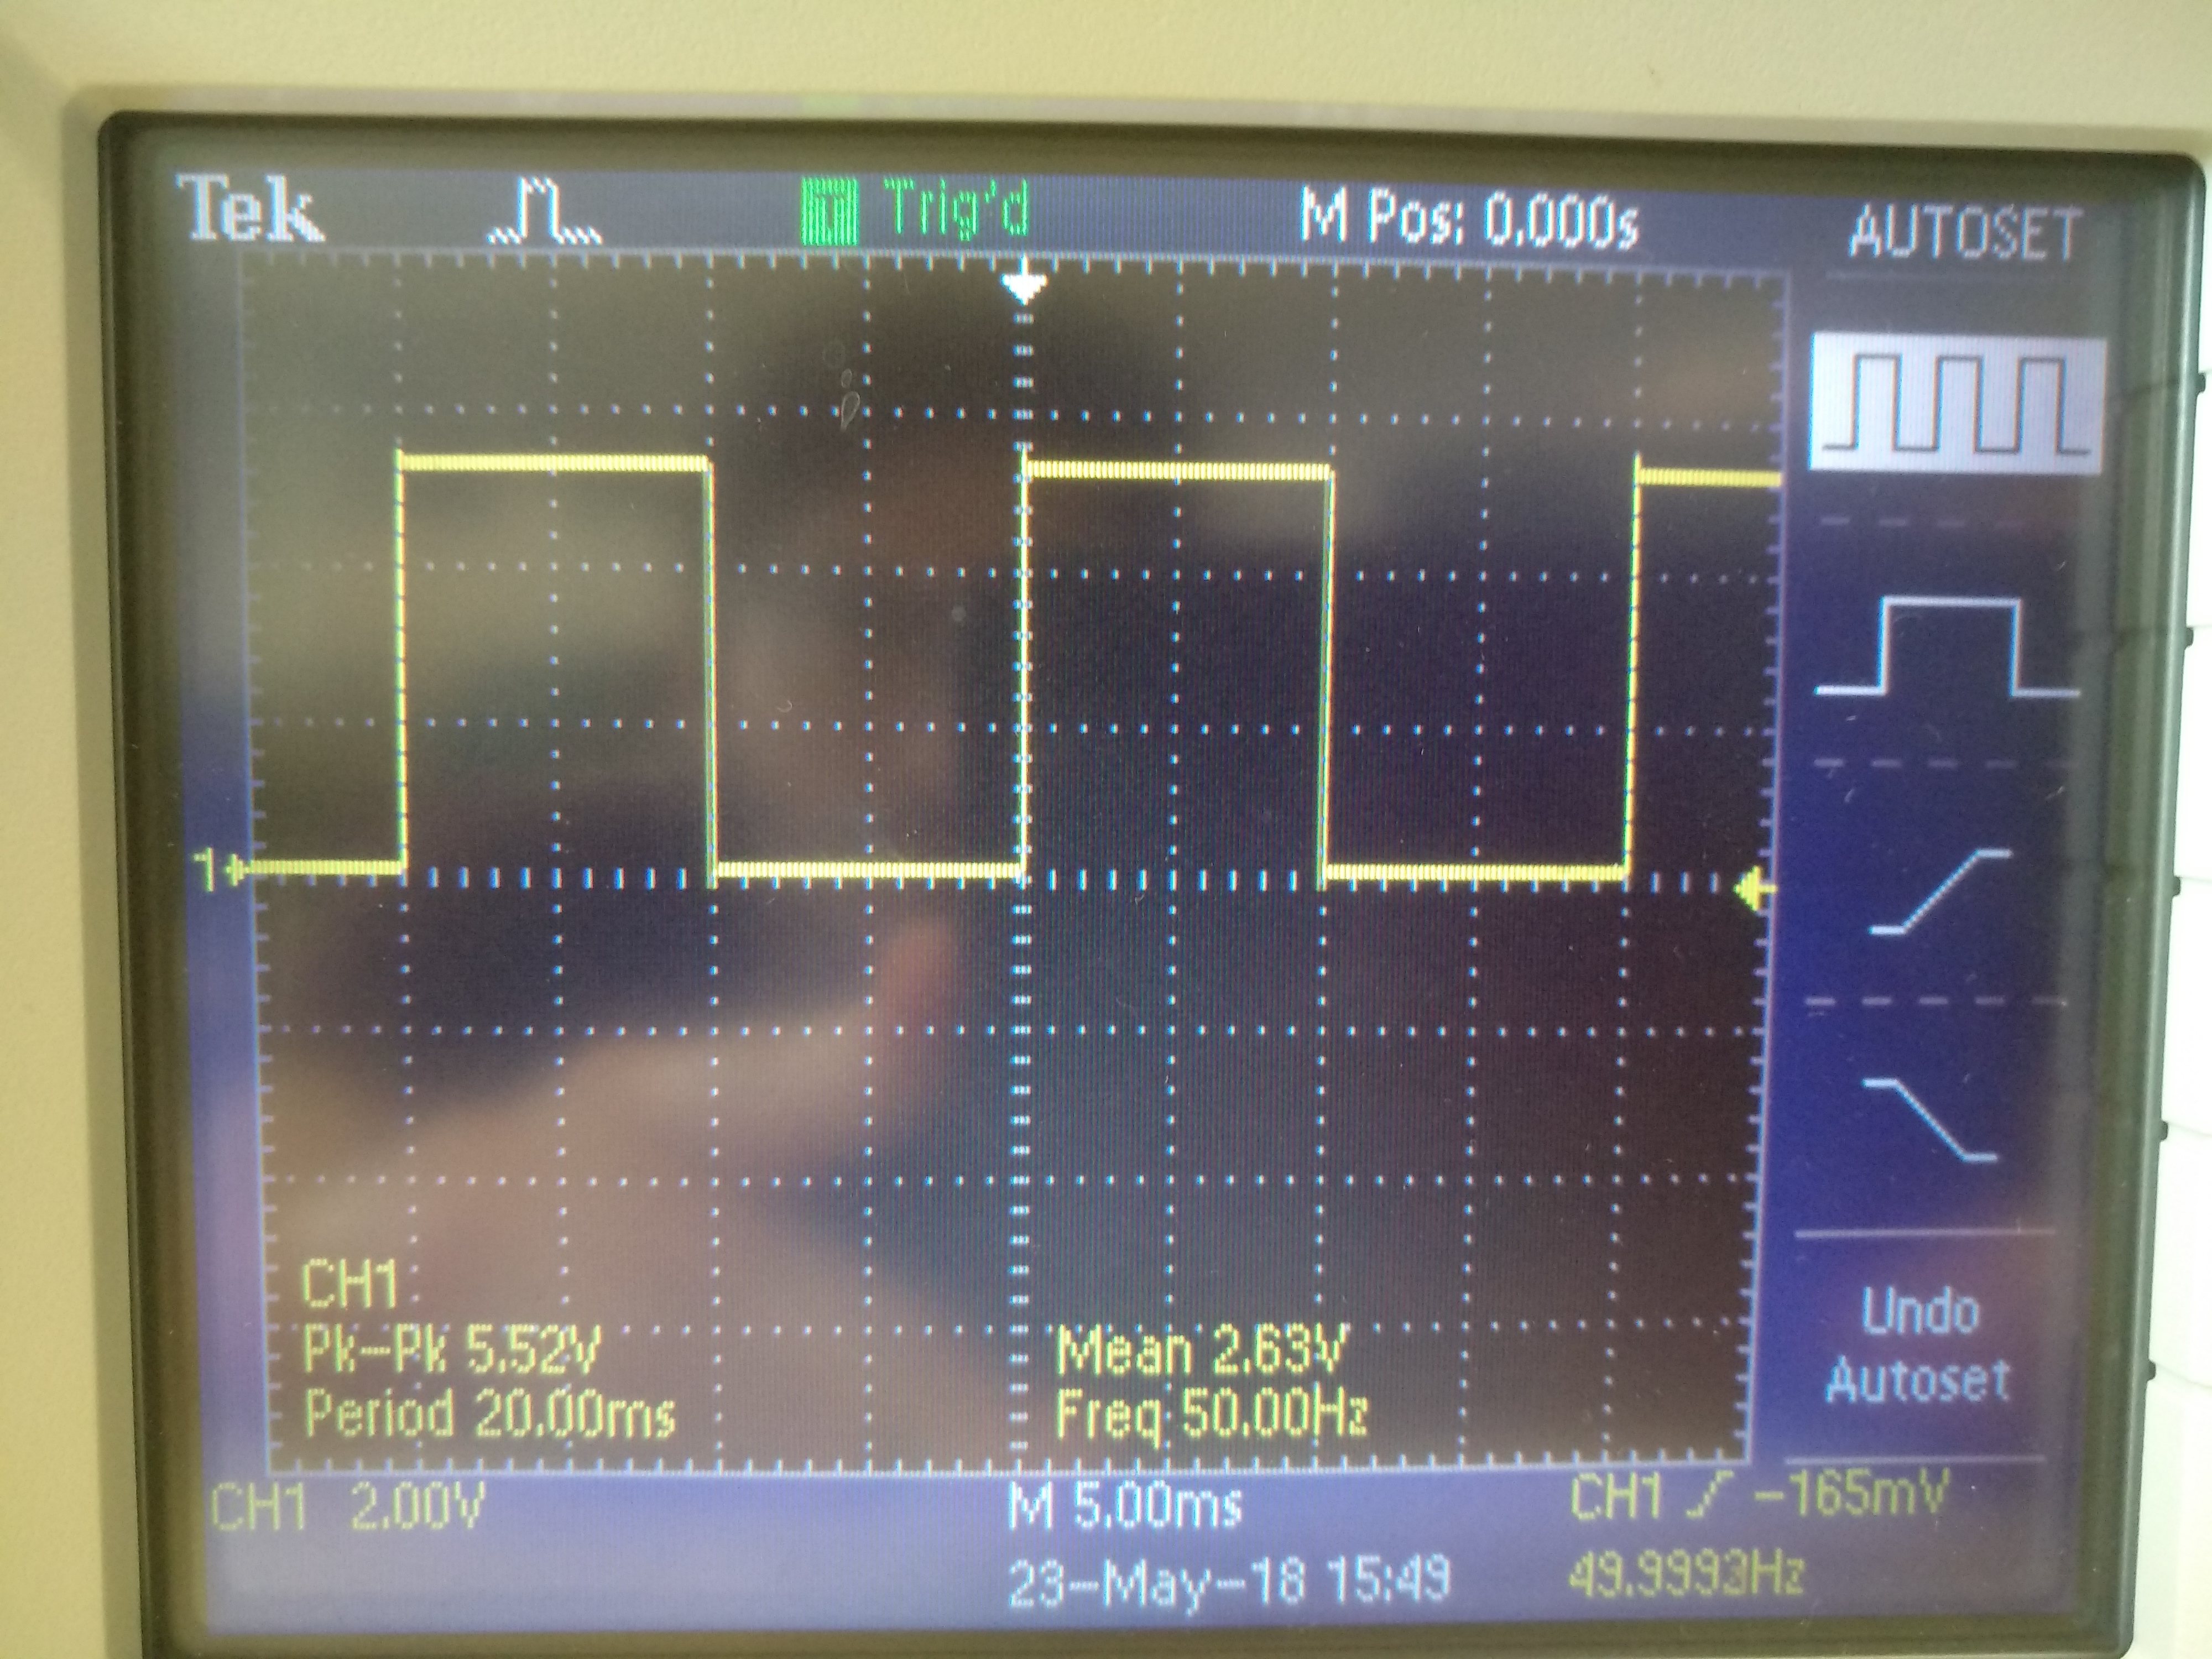
\includegraphics[width=0.8\textwidth]{osc-norm.jpg}
\caption{\label{fig:norm}f = 50Hz, dutycycle = 0.5 en brightness= 100\%.}
\end{figure}

\begin{figure}[H]
\centering
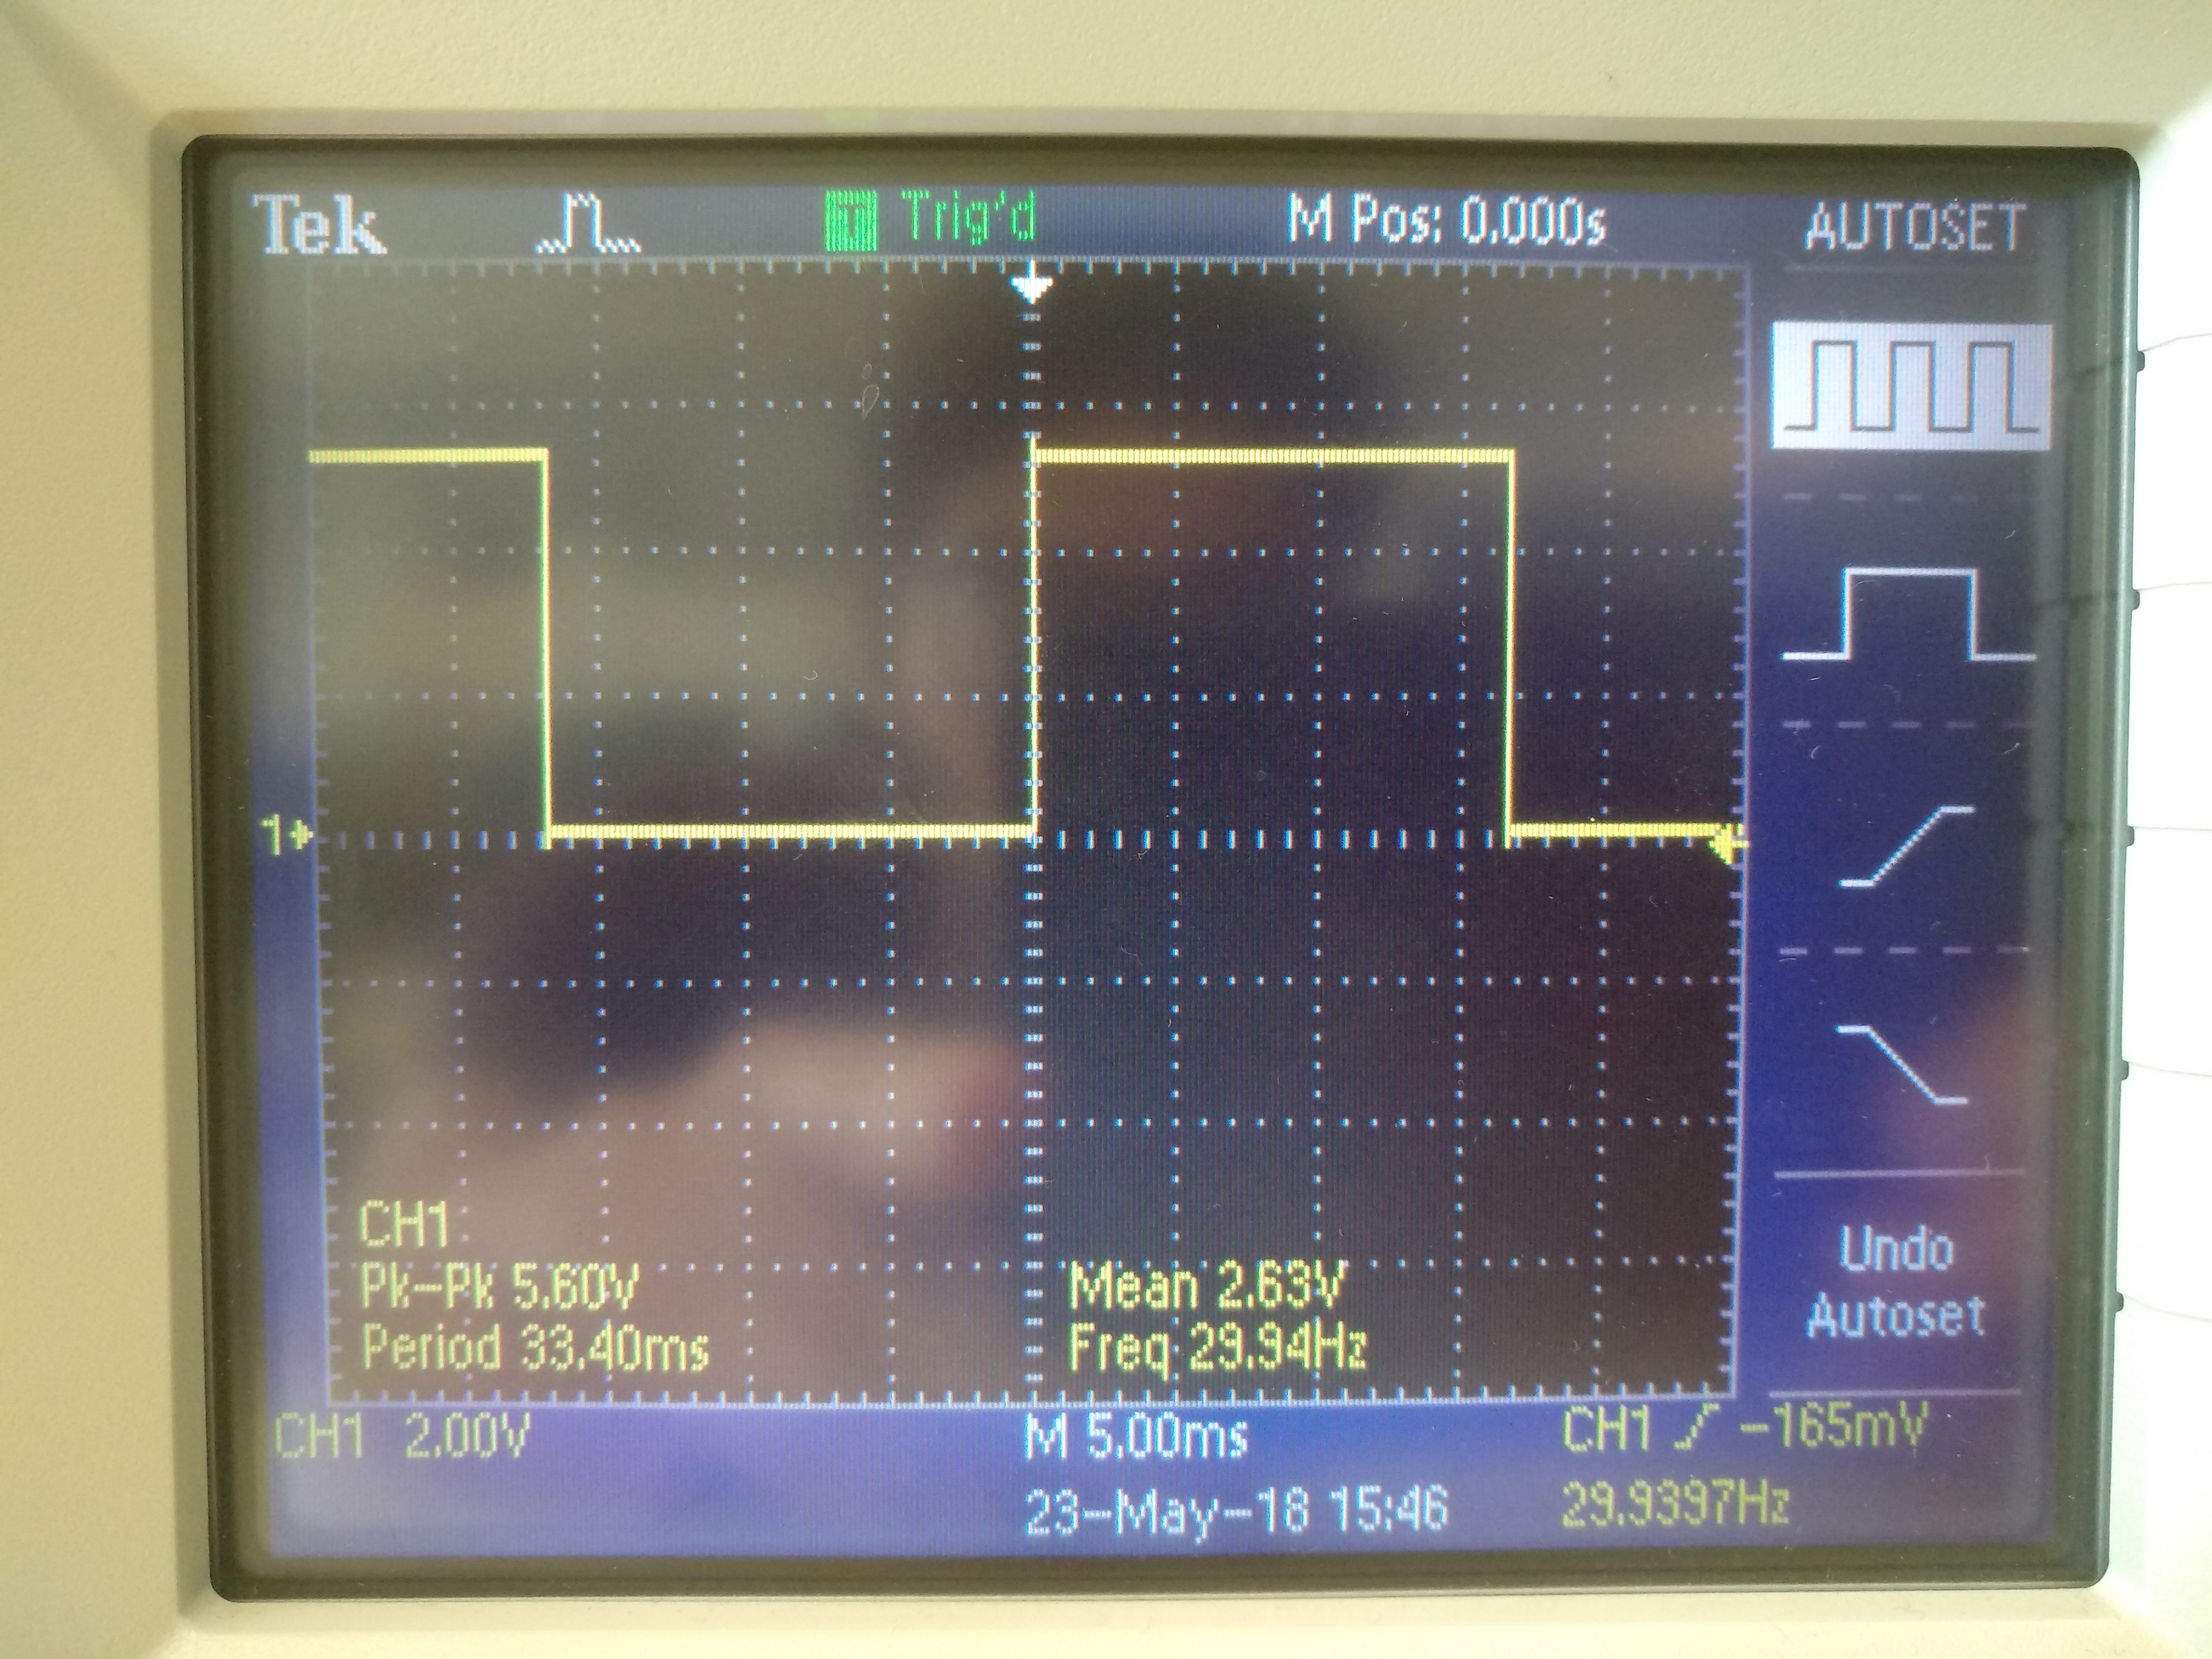
\includegraphics[width=0.8\textwidth]{osc-freq-laag.jpg}
\caption{\label{fig:frlg}f = 30Hz, dutycycle = 0.5 en brightness= 100\%.}
\end{figure}

\begin{figure}[H]
\centering
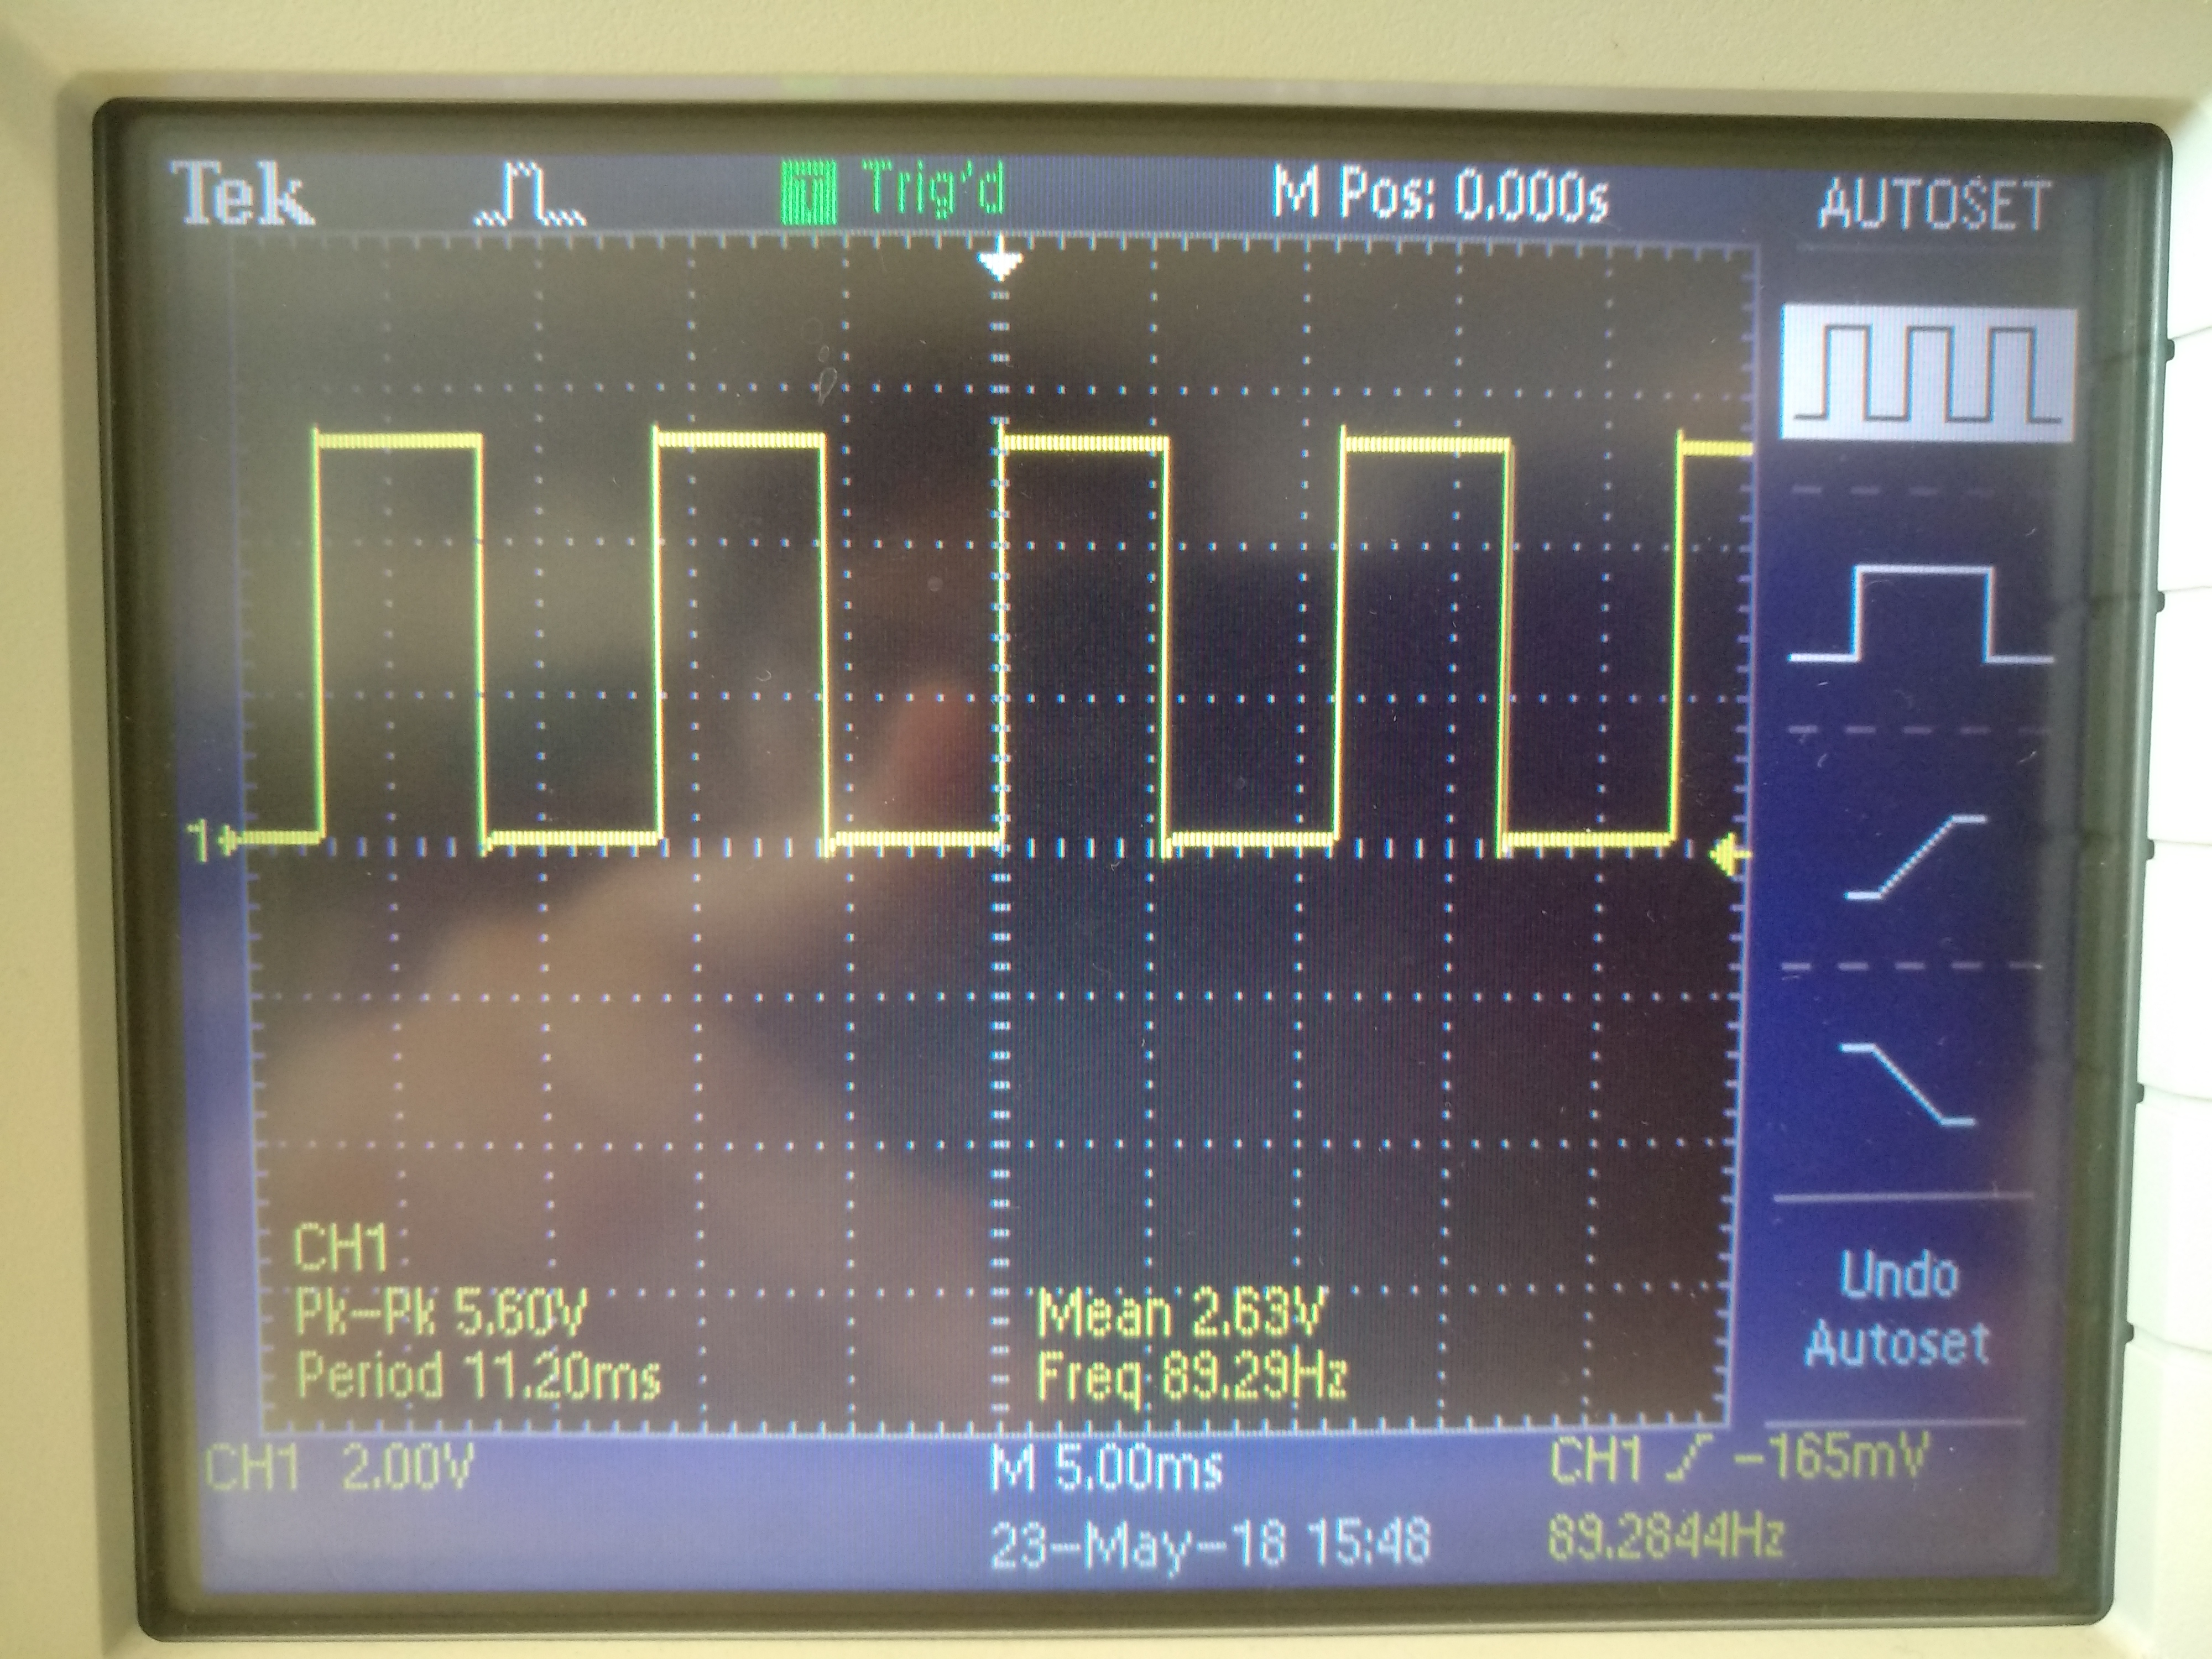
\includegraphics[width=0.8\textwidth]{osc-freq-hoog.jpg}
\caption{\label{fig:frhgfso}f = 90Hz, dutycycle = 0.5 en brightness= 100\%.}
\end{figure}

\begin{figure}[h]
\centering
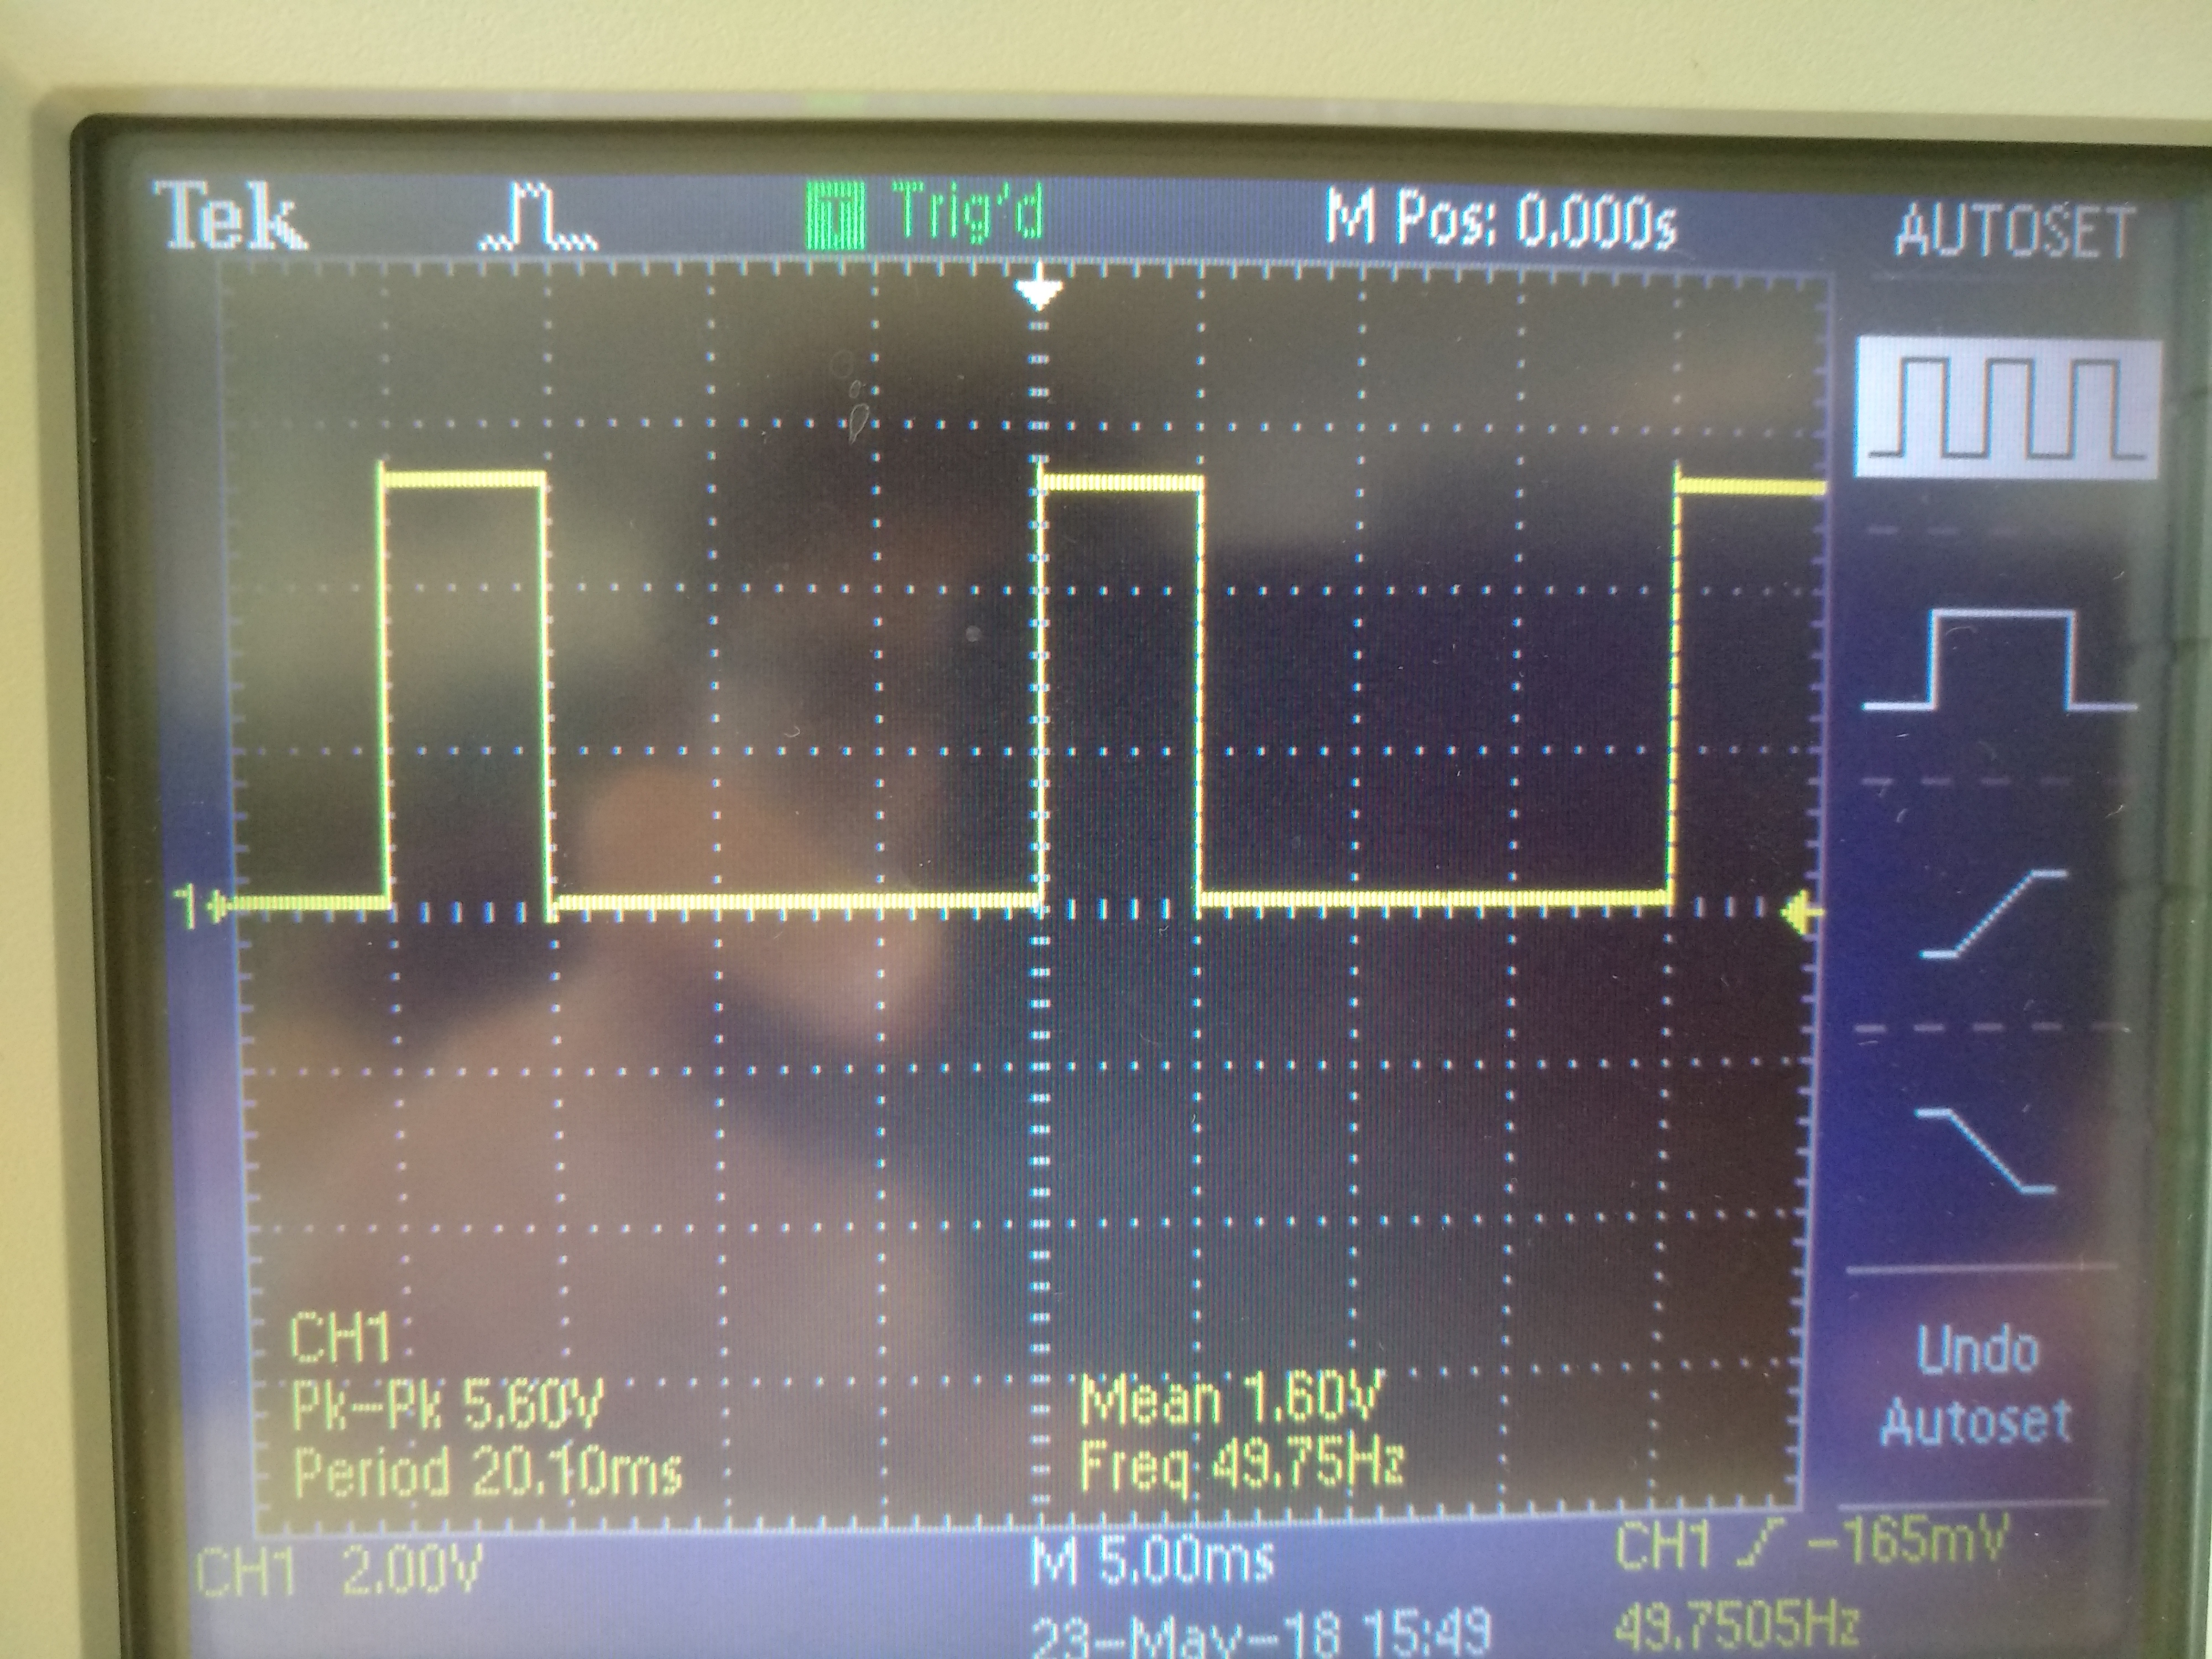
\includegraphics[width=0.8\textwidth]{osc-duty-laag.jpg}
\caption{\label{fig:dula}f = 50Hz, dutycycle = 0.25 en brightness= 100\%.}
\end{figure}

\begin{figure}[H]
\centering
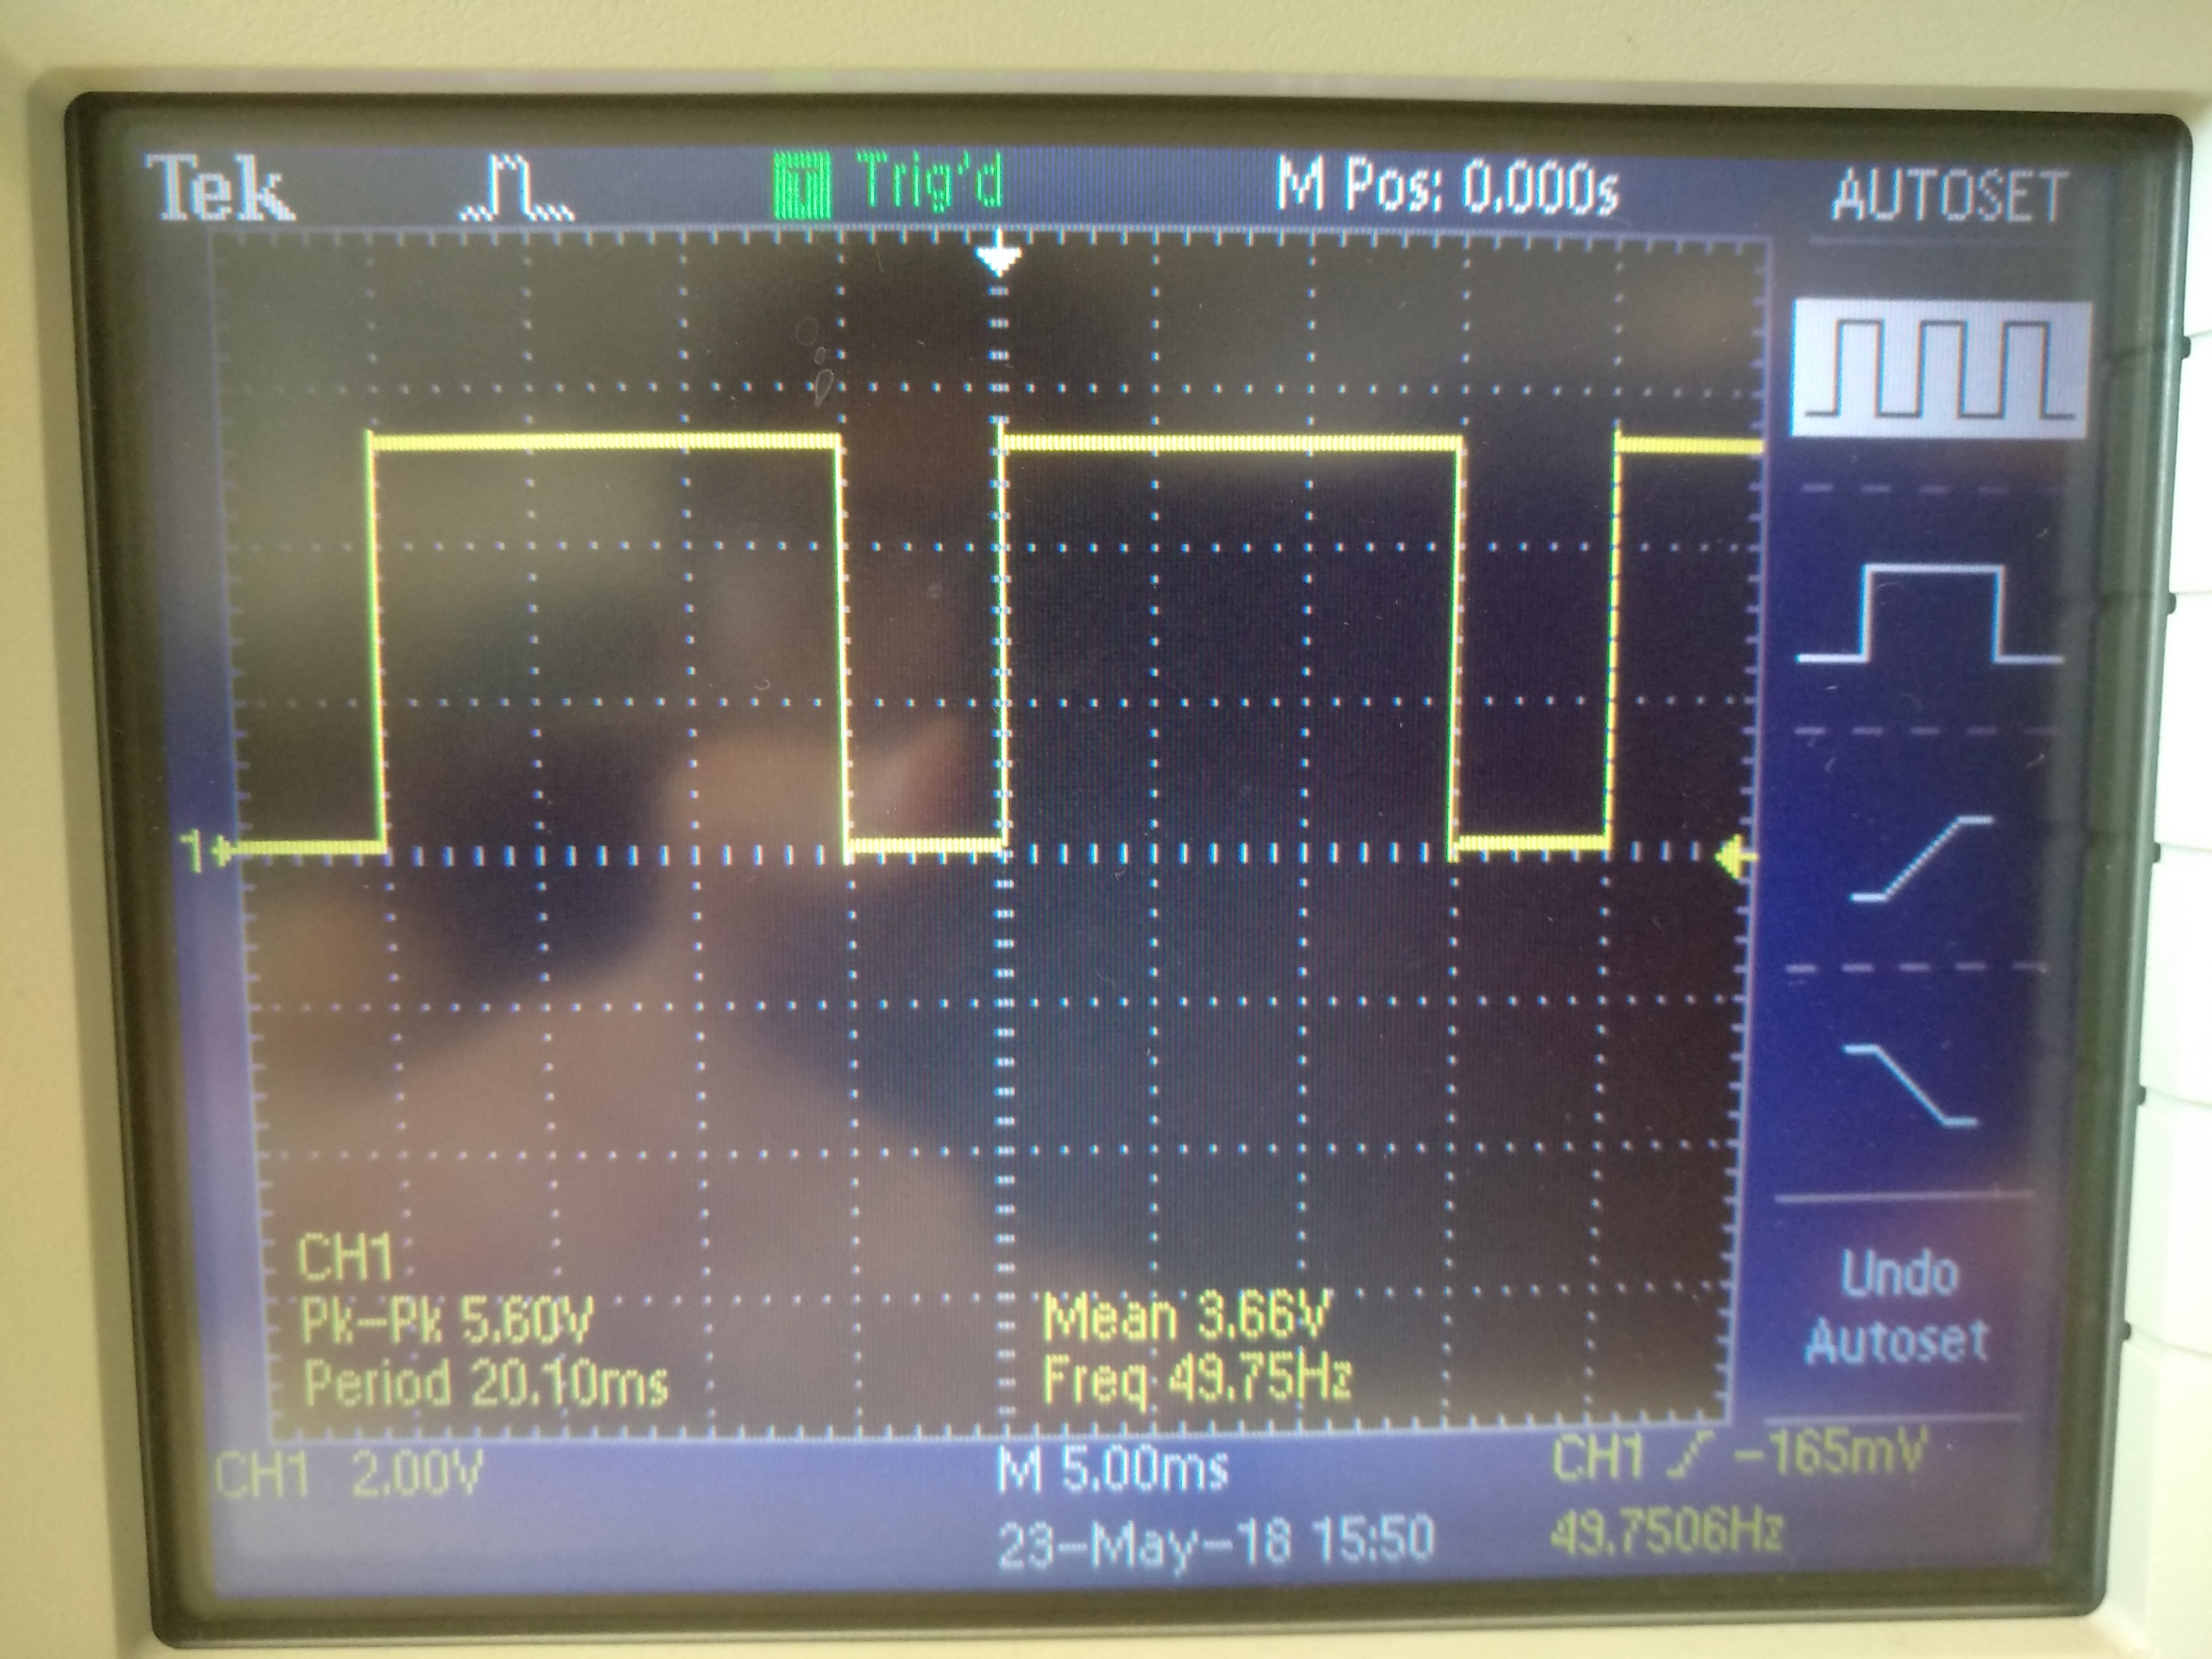
\includegraphics[width=0.8\textwidth]{osc-duty-hoog.jpg}
\caption{\label{fig:fsfdsf}f = 50Hz, dutycycle = 0.75 en brightness= 100\%.}
\end{figure}

\begin{figure}[H]
\centering
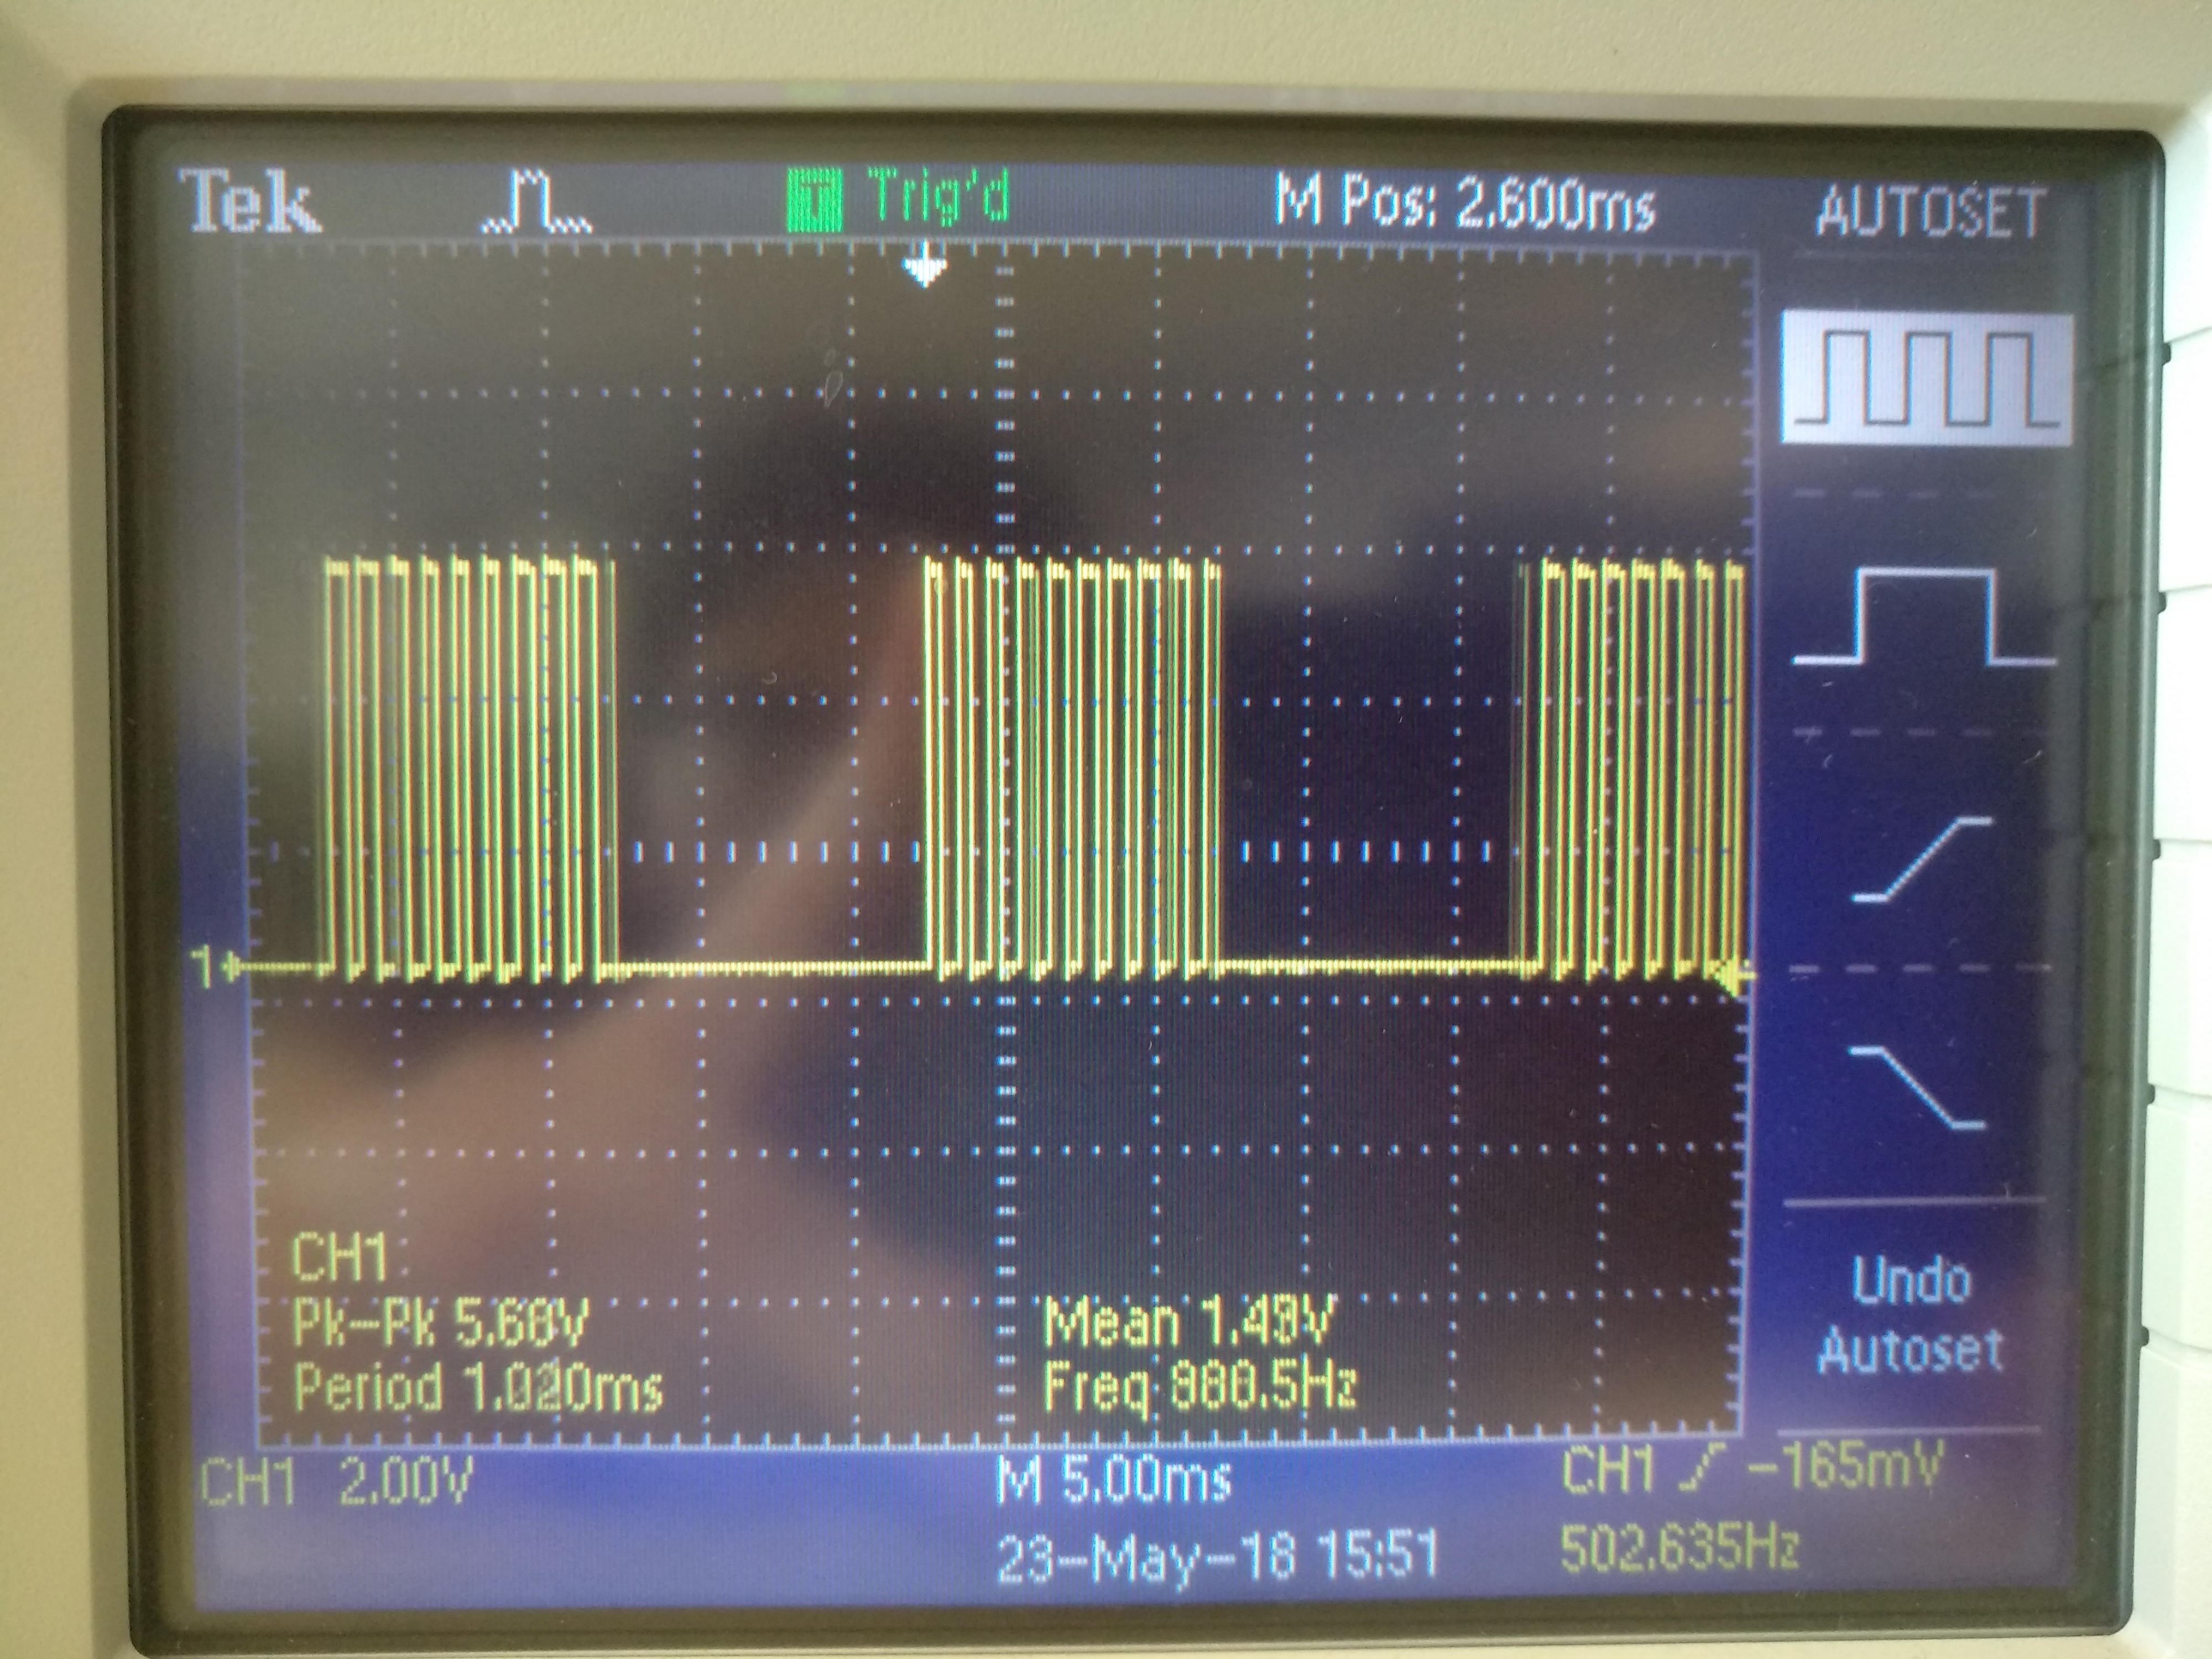
\includegraphics[width=0.8\textwidth]{osc-pwm.jpg}
\caption{\label{fig:zerze}f = 50Hz, dutycycle = 0.5 en brightness= 50\%.}
\end{figure}

\pagebreak

\section{Schema's}
\label{appendix:schema}
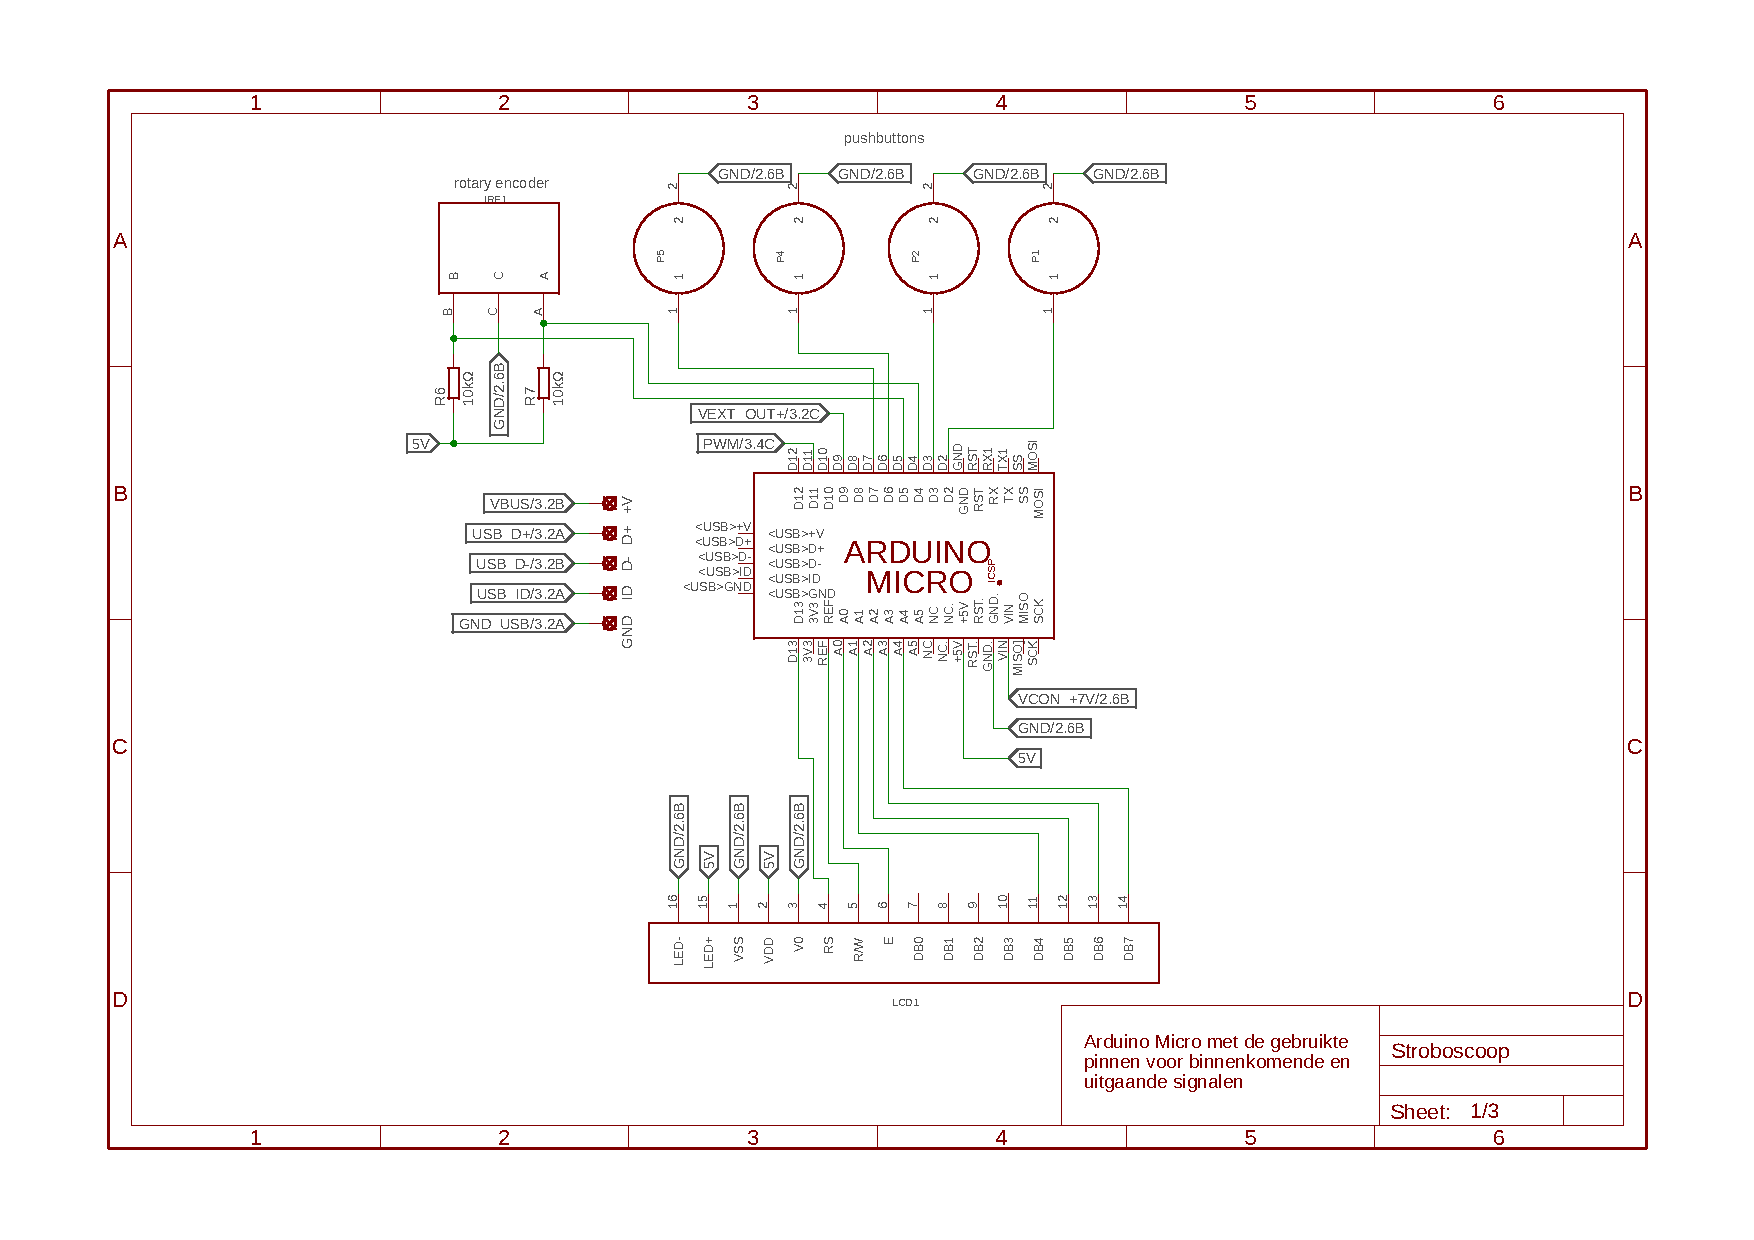
\includepdf[pages=-, landscape=true]{Stroboscoop_schema.pdf}

\section{PCB top layer}
\label{appendix:top}
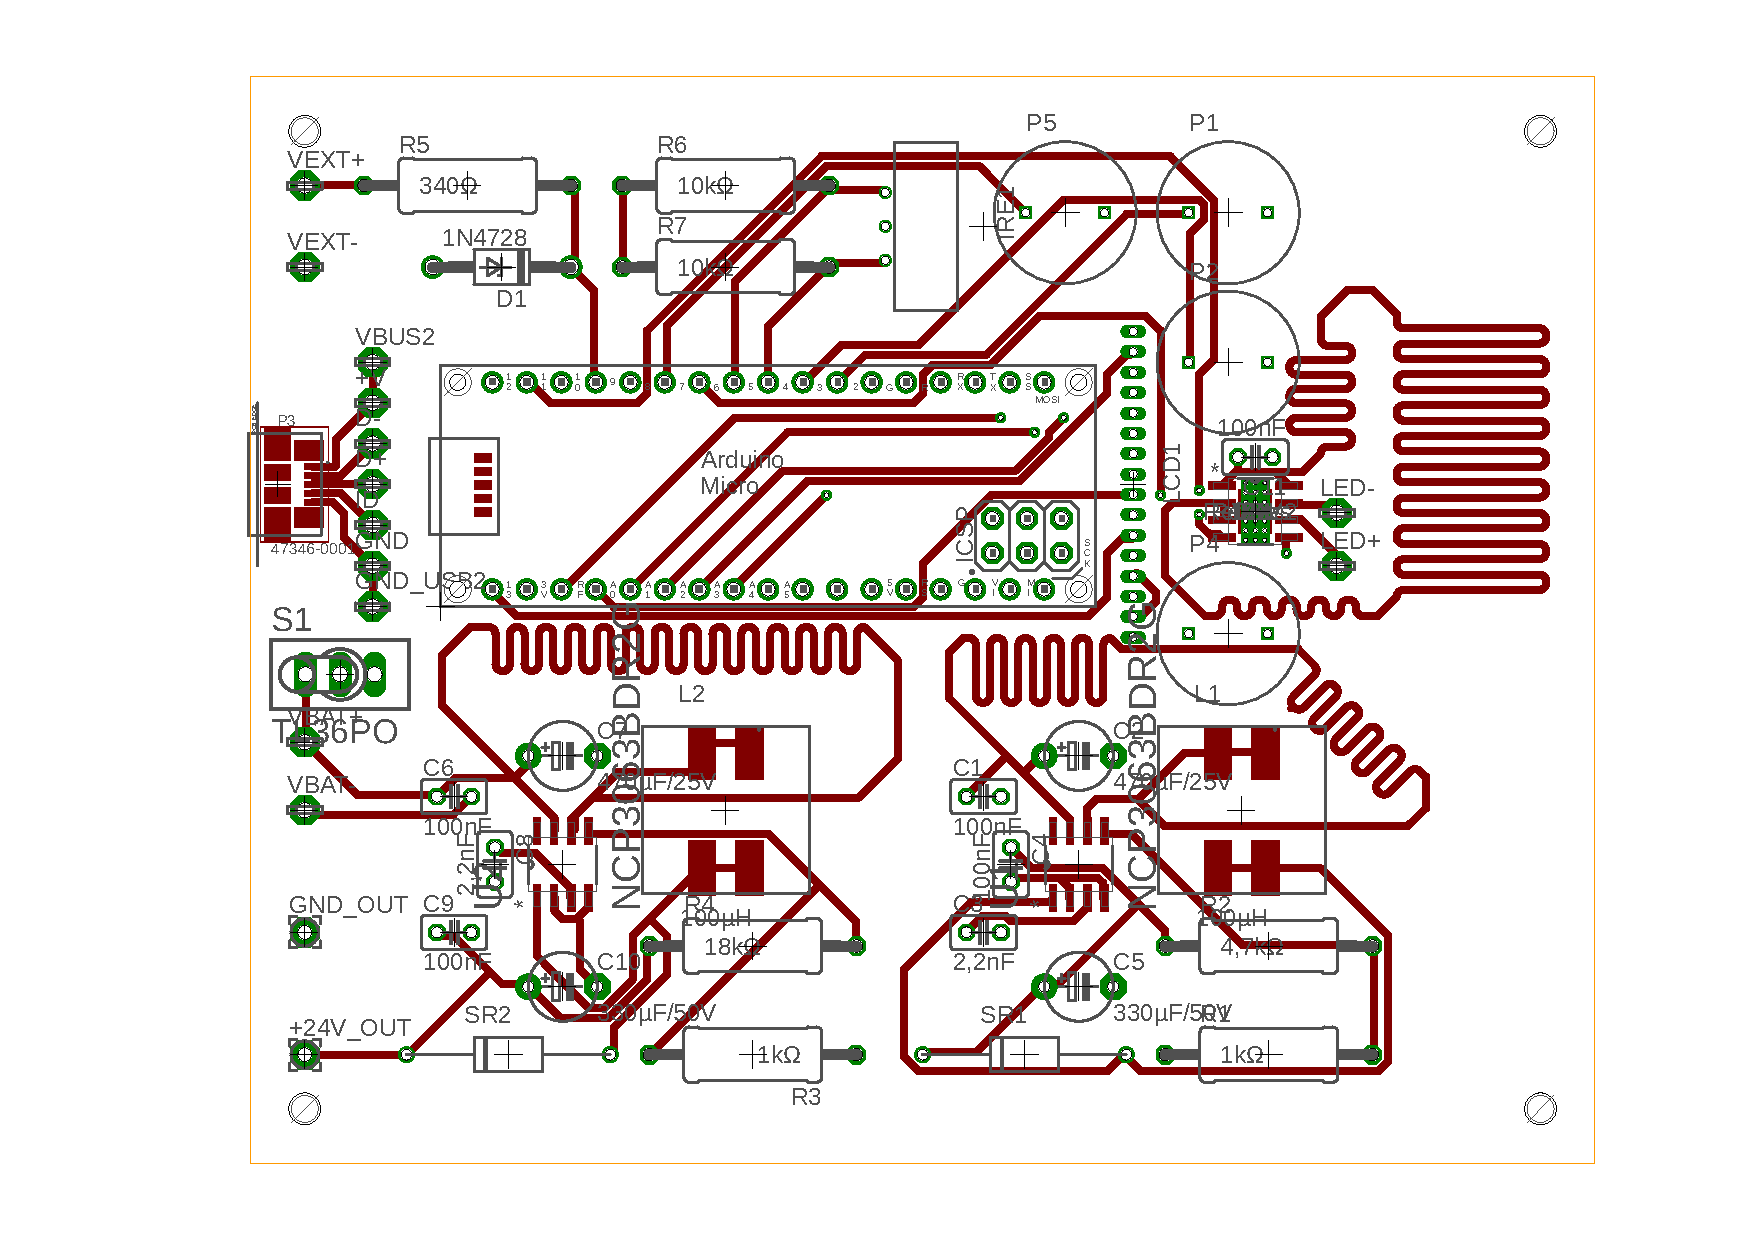
\includepdf[pages=-, landscape=true]{Top_layer.pdf}

\section{PCB bottom layer}
\label{appendix:bot}
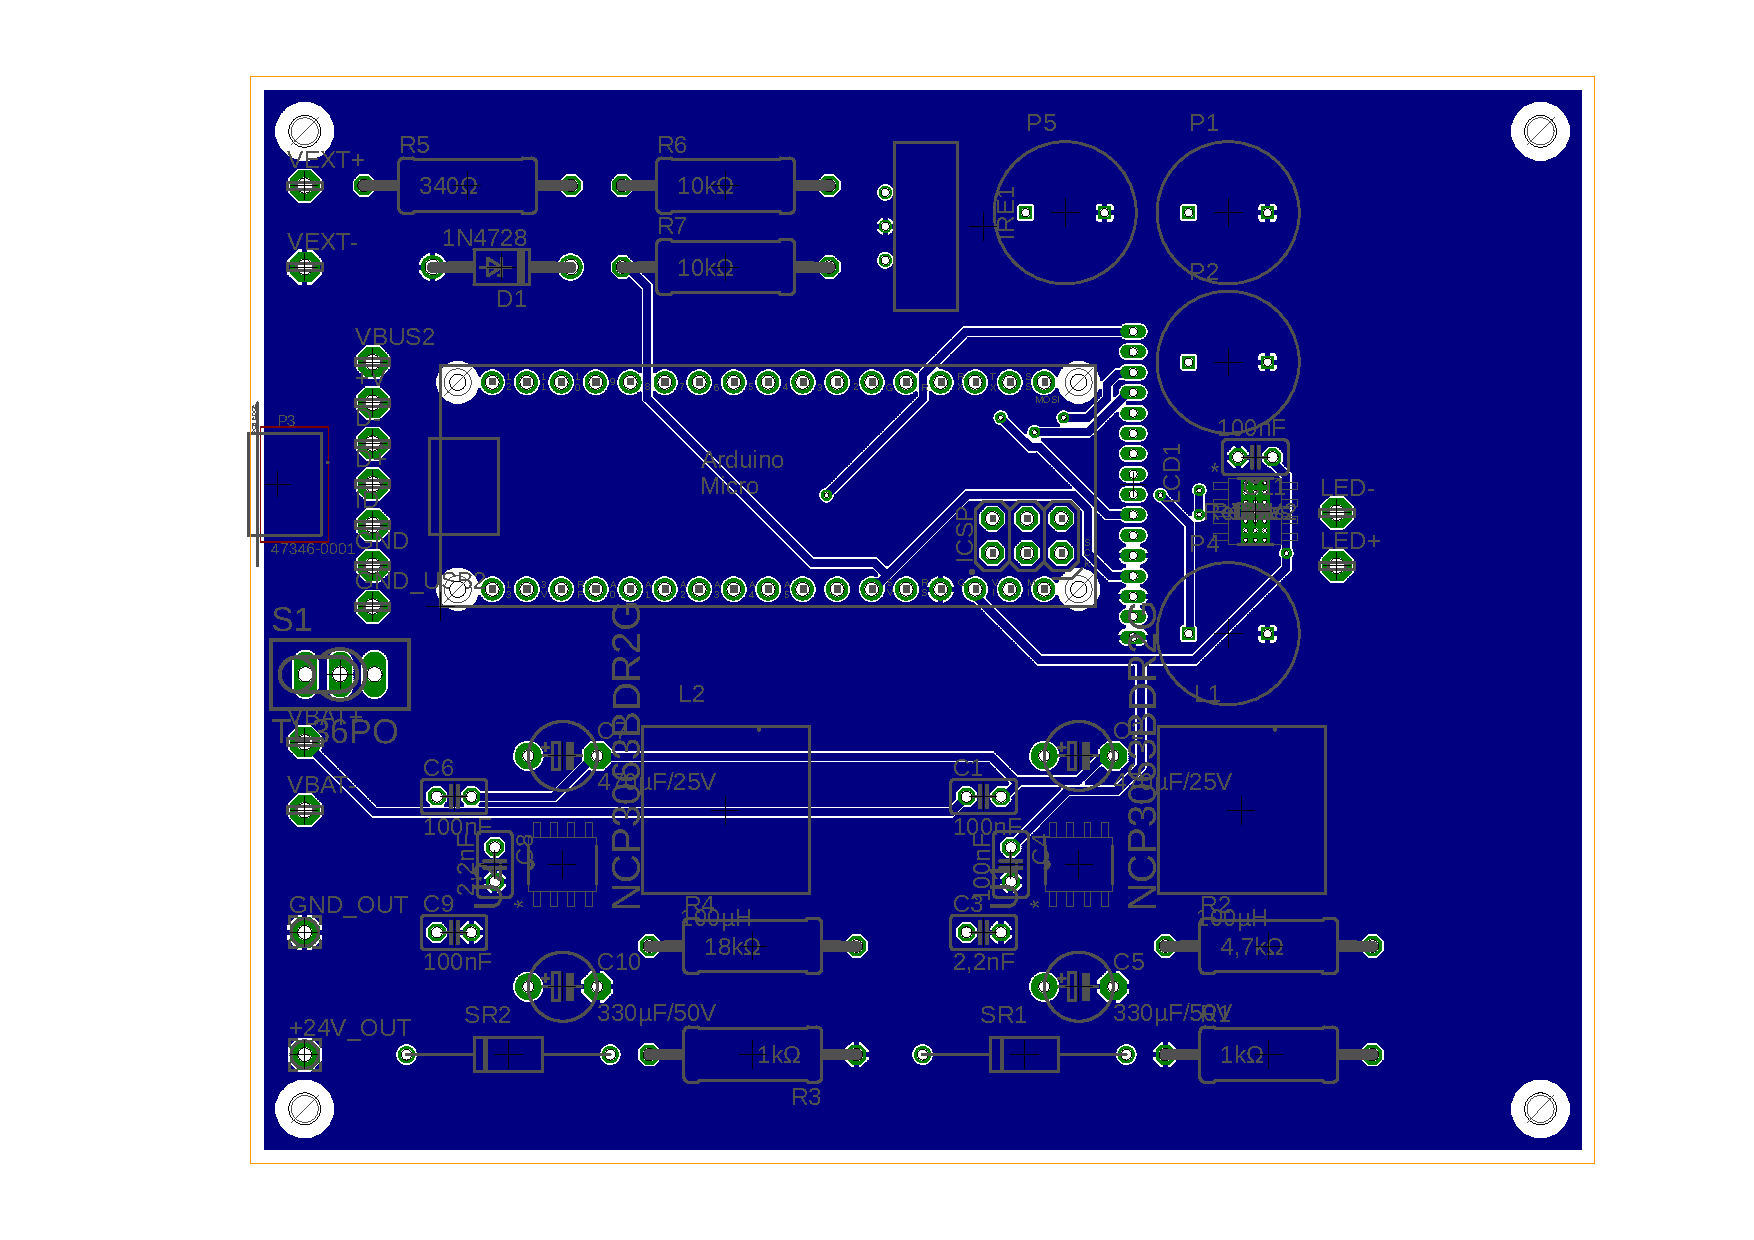
\includepdf[pages=-, landscape=true]{Bottom_layer.pdf}

\pagebreak

\section{Flowcharts}
\label{appendix:flowchart}
\begin{figure}[H]
\centering
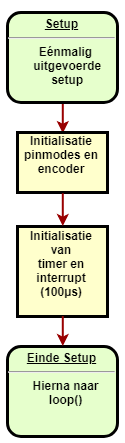
\includegraphics[width=0.2\textwidth]{Setup.png}
\caption{\label{fig:setup}Setup in pseudo-code.}
\end{figure}

\begin{figure}[H]
\centering
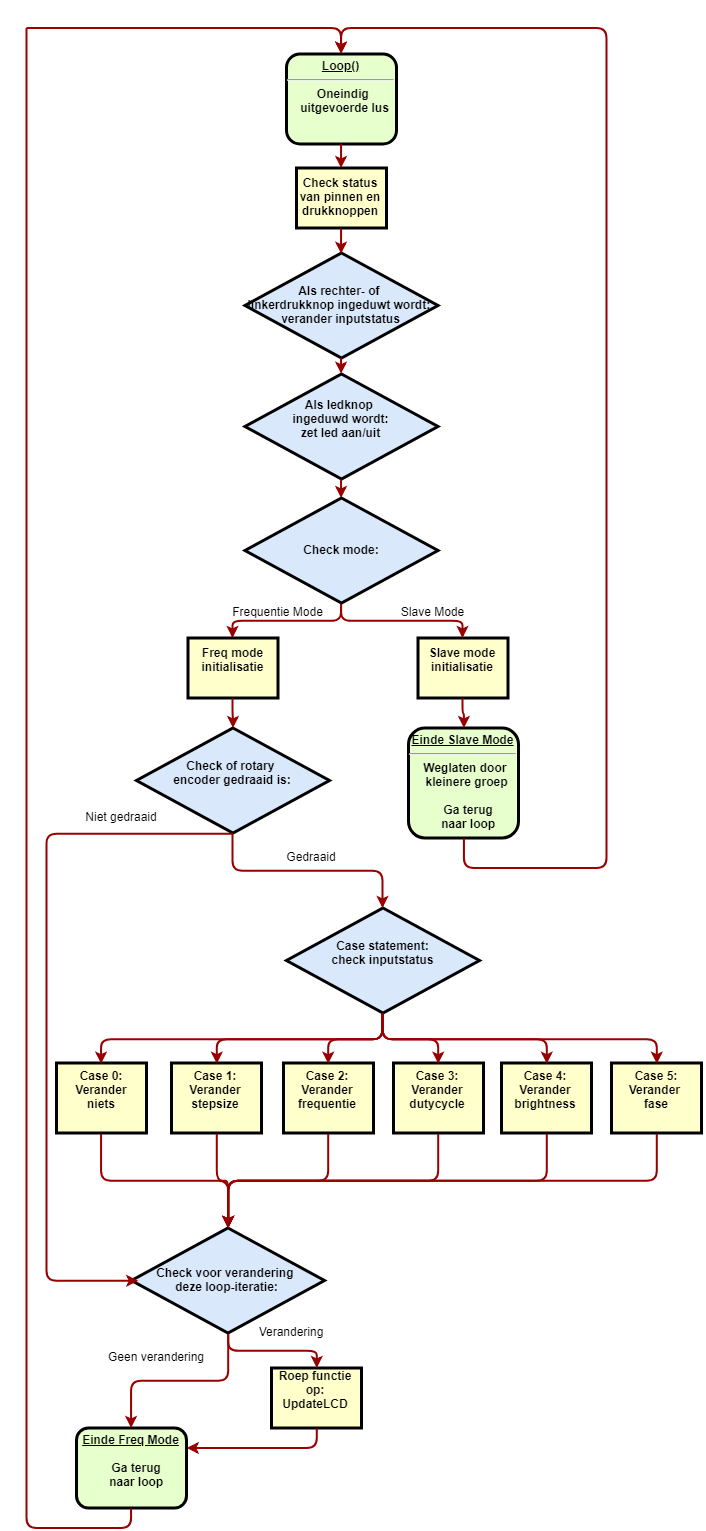
\includegraphics[width=0.75\textwidth]{Loop.png}
\caption{\label{fig:loop}Loop in pseudo-code.}
\end{figure}

\begin{figure}[H]
\centering
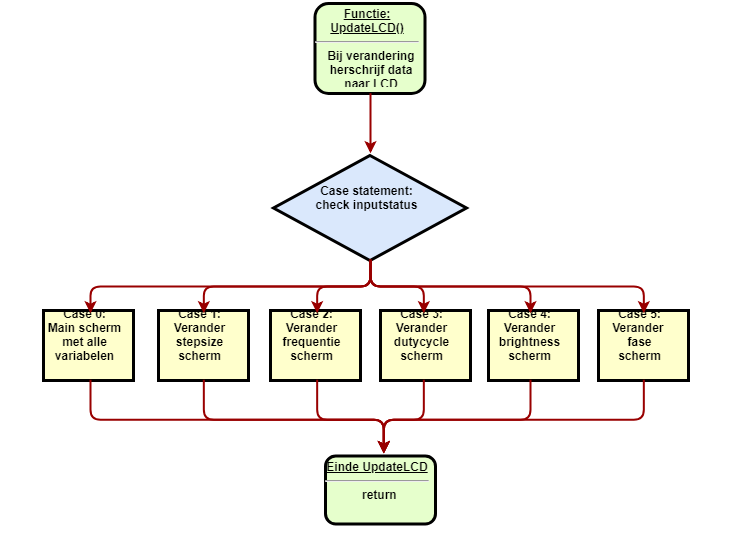
\includegraphics[width=0.7\textwidth]{UpdateLCD.png}
\caption{\label{fig:lcd}UpdateLCD function in pseudo-code.}
\end{figure}

\begin{figure}[H]
\centering
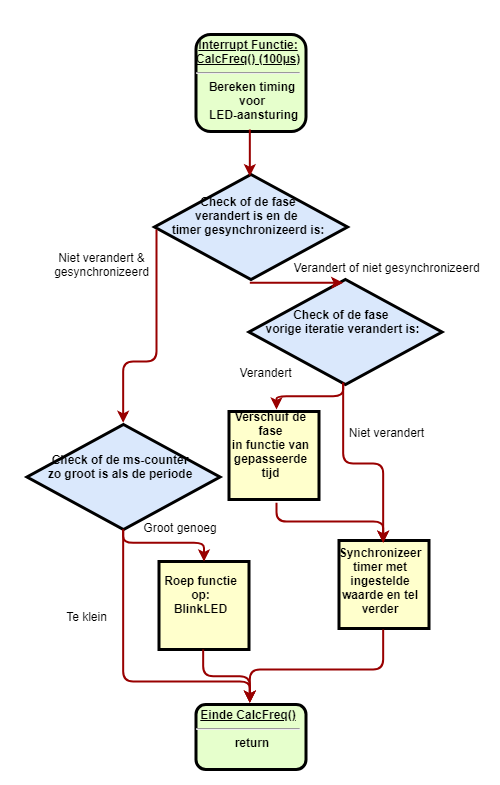
\includegraphics[width=0.5\textwidth]{Interrupt.png}
\caption{\label{fig:interrupt}100 µs interrupt function in pseudo-code.}
\end{figure}

\begin{figure}[H]
\centering
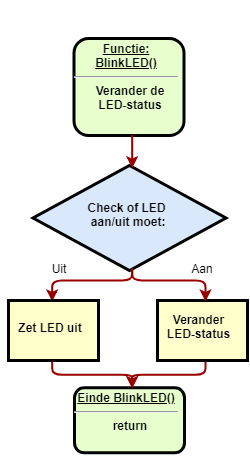
\includegraphics[width=0.3\textwidth]{blinkLED.png}
\caption{\label{fig:blinkled}BlinkLED function in pseudo-code.}
\end{figure}

\pagebreak

\section{Variabel map}
\label{appendix:vmap}
\begin{figure}[H]
\centering
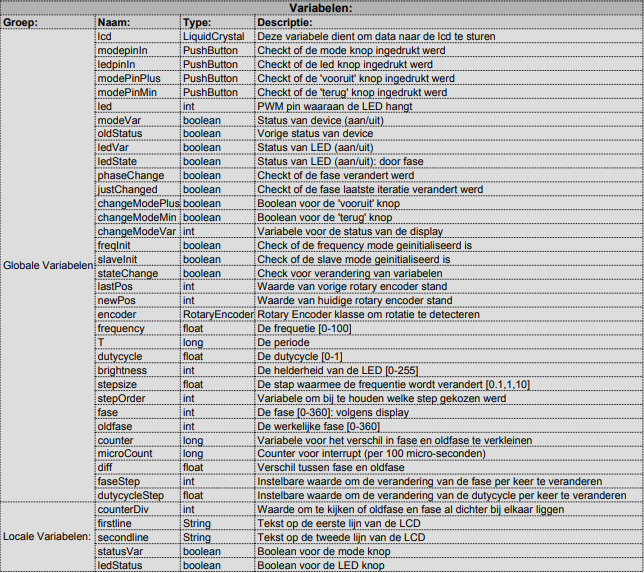
\includegraphics[width=1\textwidth]{varmap.png}
\caption{\label{fig:varmap}Variable map.}
\end{figure}

\end{appendices}

\end{document}